% !TeX program = pdflatex
% =====================================================================
%  CS5055 - Internet of Things (2026-2) · Informe P2
%  Compilar dos veces: pdflatex informe_p2.tex
% =====================================================================
\documentclass[10pt,a4paper]{article}

\usepackage[utf8]{inputenc}
\usepackage[T1]{fontenc}
\usepackage[spanish,es-noquoting,es-tabla]{babel}
\usepackage[left=1.8cm,right=1.8cm,top=1.6cm,bottom=1.8cm]{geometry}
\usepackage{lmodern}
\renewcommand{\familydefault}{\sfdefault}
\usepackage{booktabs,array,tabularx,microtype,xcolor,enumitem,titlesec,fancyhdr,graphicx,float}
\usepackage[font=small,labelfont=bf]{caption}
\usepackage{subcaption}
\usepackage{fancyvrb}
\usepackage{tikz}
\usetikzlibrary{arrows.meta,positioning,shapes.geometric,fit,calc,backgrounds}
\usepackage{pgfplots}
\pgfplotsset{compat=1.18}
\usepackage{hyperref}
\hypersetup{colorlinks=true,linkcolor=black,citecolor=blue!55!black,urlcolor=blue!55!black}

\titleformat{\section}{\large\bfseries}{\thesection.}{0.5em}{}
\titleformat{\subsection}{\normalsize\bfseries}{\thesubsection}{0.5em}{}
\titlespacing*{\section}{0pt}{10pt}{4pt}
\titlespacing*{\subsection}{0pt}{7pt}{3pt}
\setlength{\parskip}{3pt}
\setlength{\parindent}{0pt}
\renewcommand{\arraystretch}{1.15}
\setlist{itemsep=1pt,topsep=2pt}

\pagestyle{fancy}
\fancyhf{}
\renewcommand{\headrulewidth}{0pt}
\fancyfoot[C]{\scriptsize\color{black!55}CS5055 Internet of Things $\cdot$ Informe P2 $\cdot$ \thepage}

\newcolumntype{L}[1]{>{\raggedright\arraybackslash}p{#1}}
\newcolumntype{C}[1]{>{\centering\arraybackslash}p{#1}}
\newcommand{\cod}[1]{\texttt{\small #1}}
\newcommand{\COd}{CO\textsubscript{2}}

% Estilos de diagramas (sobrios: color solo para agrupar)
\tikzset{
  blk/.style={draw=black!70,rounded corners=2pt,align=center,font=\scriptsize,inner sep=3pt,fill=white},
  grp/.style={draw=black!35,dashed,rounded corners=4pt,inner sep=5pt},
  grplbl/.style={font=\scriptsize\bfseries,text=black!65},
  arr/.style={-{Stealth[length=4pt]},black!70},
  pw/.style={-{Stealth[length=4pt]},red!65!black,thick},
  lbl/.style={font=\tiny,text=black!70,fill=white,inner sep=1pt},
  term/.style={draw=black!70,rounded corners=8pt,align=center,font=\scriptsize,fill=black!5,inner sep=3pt},
  proc/.style={draw=black!70,align=center,font=\scriptsize,inner sep=3pt,fill=white,text width=3.3cm},
  dec/.style={draw=black!70,diamond,aspect=3,align=center,font=\scriptsize,inner sep=0pt,fill=black!4},
}

\begin{document}

% ------------------------------------------------------------------ Carátula
\begin{titlepage}
\thispagestyle{empty}
\centering
\vspace*{1.5cm}

\includegraphics[width=5.3cm]{descarga.png}\par
\vspace{1.9cm}
{\large\bfseries Informe Proyecto\par}
\vspace{0.8cm}
{\Huge\bfseries Calienfriito\par}
\vspace{0.6cm}
{\LARGE\bfseries Nodo IoT de control térmico y calidad de aire para aulas\par}
\vspace{1cm}
{\large Reglas locales y control predictivo con un modelo preentrenado:\par}
{\large diseño, implementación y validación\par}
\vspace{1.5cm}
{\normalsize\bfseries Curso\par}
{\normalsize Internet of Things (CS5055) $\cdot$ 2026-2\par}
\vspace{0.6cm}
{\normalsize\bfseries Equipo\par}
{\normalsize Balcazar Santa Cruz, Kiara Alexandra\par}
{\normalsize Carlos Acosta, Rodrigo Dion\par}
{\normalsize Gomero Castillo, Brayan Eduardo\par}
\vspace{0.6cm}
{\normalsize\bfseries Profesores\par}
{\normalsize Arias Obregon, Gabriel Andres\par}
{\normalsize Williams Valencia, Carlos Eduardo\par}
\vspace{0.45cm}
{\normalsize\bfseries TA\par}
{\normalsize Chavez Balarezo, Fabricio\par}
\vfill
{\normalsize 14 de noviembre de 2026\par}
\end{titlepage}

% ===================================================================== 1
\section{Título del proyecto propuesto}
\textbf{Calienfriito}: nodo IoT de bajo costo que mide temperatura, humedad, calidad de aire (\COd{}) y monóxido de carbono (CO) en un aula, decide localmente si ventilar o dar la alarma, y publica su estado por MQTT a una plataforma en la nube donde una segunda lógica, basada en aprendizaje, se evalúa en paralelo contra las reglas del nodo. Como adicional al proyecto, el equipo integró una ESP32-CAM independiente para aportar un conteo visual de ocupación al modelo de ML; el control térmico y la seguridad local siguen siendo el foco principal.

% ===================================================================== 2
\section{Introducción, problemática y marco teórico}
\subsection{Introducción}
En edificios como el de UTEC, el aire acondicionado se gobierna desde un sistema central (BMS, \emph{Building Management System}) que trabaja por zonas o por piso. Ese sistema no sabe cuántas personas hay en cada salón ni cómo cambia el aire dentro de él, por lo que las decisiones se toman con información agregada. Calienfriito agrega a cada aula su propio lazo de control: sensores que miden lo que pasa adentro, un microcontrolador que decide en el lugar y actuadores de baja tensión que responden de inmediato, más una plataforma web que reúne la información de todas las aulas.

El proyecto también plantea una pregunta de ingeniería: \emph{¿pronosticar la temperatura del aula con un modelo de IA preentrenado y encender el ventilador antes de que suba reduce el tiempo de incomodidad por calor frente a reglas de umbral?} En lugar de asumir la respuesta, ambas lógicas corren sobre los mismos datos y se comparan por los minutos de clase sobre 24,5\,$^\circ$C, además de la energía (sección~\ref{sec:resultados}).

\subsection{Problemática}
\begin{itemize}[leftmargin=12pt]
  \item \textbf{La climatización ignora la ocupación.} La carga térmica de un aula crece con cada persona (del orden de 100\,W por ocupante en reposo); un sistema que no la mide enfría salones vacíos y se queda corto en los llenos.
  \item \textbf{La calidad del aire no se vigila.} La concentración de \COd{} sube con la ocupación y, en niveles moderados, ya afecta la toma de decisiones de las personas~\cite{satish}; hoy no hay medición ni corrección en el aula.
  \item \textbf{No hay detección local de monóxido de carbono.} Una fuga de CO no tiene sensor ni respuesta automática en el salón.
\end{itemize}

\subsection{Marco teórico}
\textbf{Ocupación a partir del \COd{} y visión.} Las personas exhalan \COd{} a una tasa casi constante; con un balance de masa en el volumen del aula, el aumento de concentración sobre el nivel exterior ($\approx$\,420\,ppm) permite estimar la ocupación sin cámaras~\cite{batterman}. En este proyecto el MQ-135 se usa como indicador \emph{relativo} de esa concentración. Como canal complementario, la ESP32-CAM publica \cod{people\_count} y \cod{confidence} en \cod{ccs/<aula>/occupancy}; el backend puede reemplazar la estimación por CO$_2$ o ponderarla durante la calibración.

\textbf{Ventilación forzada y confort.} Mover aire sobre las personas aumenta la pérdida de calor por convección; en aulas con ventiladores se mantiene el confort a temperaturas más altas y se observan efectos en el desempeño cognitivo~\cite{cen}.

\textbf{Histéresis y tiempo mínimo de conmutación.} Un controlador de dos posiciones con un solo umbral oscila (\emph{short cycling}) y desgasta motores y relés. La práctica habitual en climatización es usar una banda muerta y un tiempo mínimo entre cambios~\cite{shafrir}. Calienfriito usa una banda de $\pm0{,}5\,^\circ$C alrededor de 24\,$^\circ$C y un mínimo de 60\,s entre cambios de actuador.

\textbf{MQTT.} Protocolo publicación/suscripción ligero sobre TCP. Se usan tres de sus mecanismos: QoS~1 (entrega al menos una vez), mensajes retenidos (el último comando sobrevive a un reinicio del nodo) y \emph{Last Will} (el broker publica \cod{offline} si el nodo deja de responder).

\textbf{Sensores de gas MOS.} El MQ-135 y el MQ-7 cambian su resistencia con la concentración del gas y necesitan precalentamiento y calibración~\cite{rawdhan}; su salida analógica de 0--5\,V se adapta al ADC de 3,3\,V del ESP32 con un divisor resistivo.

% ===================================================================== 3
\section{Estado del arte}
\label{sec:estado}
Se analizaron seis trabajos de 2022 a 2026 (dos por integrante), agrupados según la decisión de diseño que respaldan. La Tabla~\ref{tab:arte} resume qué aporta cada uno, qué le falta respecto a nuestro problema y qué tomamos.

\textbf{Ventilación por demanda.} Lu \emph{et al.}~\cite{lu} revisan las estrategias de ventilación controlada por \COd{} en edificios comerciales y concluyen que ahorran energía sin perder calidad de aire, pero que su desempeño depende de la calidad del sensor y de la estrategia de control. Es la base de ligar la ventilación a la ocupación estimada; su limitación para nuestro caso es que asume sensores NDIR y sistemas de edificio, no un nodo de bajo costo por aula. Por eso tratamos el MQ-135 como indicador relativo y no como medición absoluta.

\textbf{Actuación con ESP32 por WiFi.} Ni'amah \emph{et al.}~\cite{niamah} implementan un ESP32 que gobierna un ventilador por WiFi. Valida la viabilidad de la actuación remota con el mismo microcontrolador, pero el control depende de la red y no considera seguridad local. Calienfriito invierte ese orden: el nodo decide y actúa aunque la red caiga, y la nube solo observa, compara y, si se le autoriza, ordena.

\textbf{Controladores avanzados frente a reglas.} Kumkam \emph{et al.}~\cite{kumkam} comparan aprendizaje por refuerzo y control predictivo por modelo (MPC) para HVAC, y Gao y Wang~\cite{gao} comparan refuerzo con y sin modelo. Ambos muestran ganancias de energía de los métodos avanzados, pero con alto costo de entrenamiento, dependencia de simuladores detallados y resultados muy sensibles al caso de uso. De ahí tomamos dos decisiones: evitar el entrenamiento costoso usando un modelo de pronóstico \emph{preentrenado} (Chronos-Bolt~\cite{chronos}, que predice series de tiempo sin ajustarse a cada aula) dentro de un control predictivo simple, y validarlo nosotros antes de entregarle el control.

\textbf{Calibración de sensores de bajo costo.} Rawdhan y Ali~\cite{rawdhan} muestran que los MQ requieren calibración (por ejemplo, $R_0$ en aire limpio y curvas por gas) para que su lectura sea confiable. Su trabajo no aborda el uso dentro de un lazo de control; nosotros lo usamos para justificar umbrales relativos (ocupación) y un margen de seguridad amplio (alarma de CO a 50\,ppm).

\textbf{Confort, ventiladores y desempeño.} Cen \emph{et al.}~\cite{cen} miden en aulas tropicales que la ventilación asistida mantiene el confort y el rendimiento cognitivo a temperaturas mayores. Respalda usar un ventilador como actuador principal en Lima, aunque su estudio usa equipos dimensionados para el aula; nuestro resultado de la sección~\ref{sec:resultados} muestra que un ventilador de 2,4\,W no alcanza para mover la temperatura del salón.

\begin{table}[H]
\centering\scriptsize
\caption{Estado del arte: aporte, limitación frente a nuestro problema y decisión que respalda.}
\label{tab:arte}
\begin{tabularx}{\linewidth}{L{2.4cm}XXX}
\toprule
\textbf{Trabajo} & \textbf{Aporte} & \textbf{Limitación para un aula} & \textbf{Qué tomamos} \\
\midrule
Lu \emph{et al.} (2022)~\cite{lu} & Revisión de ventilación por demanda con \COd{} & Asume sensores NDIR y control de edificio & Ventilar según ocupación, MQ-135 como indicador relativo \\
Ni'amah \emph{et al.} (2026)~\cite{niamah} & ESP32 controla un ventilador por WiFi & Sin lógica local ni seguridad ante caída de red & ESP32 + WiFi, pero con decisión y alarma locales \\
Kumkam \emph{et al.} (2025)~\cite{kumkam} & RL vs. MPC en HVAC & Costo de entrenamiento y simulador detallado & Control predictivo con modelo preentrenado, evaluado en sombra \\
Gao y Wang (2023)~\cite{gao} & RL con y sin modelo & Ganancia depende del caso de uso & Validación propia antes de ceder el control \\
Rawdhan y Ali (2026)~\cite{rawdhan} & Calibración de sensores MQ & No integra el sensor en un lazo de control & Umbrales relativos y calibración en sitio \\
Cen \emph{et al.} (2024)~\cite{cen} & Ventiladores mantienen confort en aulas & Equipos dimensionados para el aula & Ventilador como actuador; dimensionarlo (sec.~\ref{sec:resultados}) \\
\bottomrule
\end{tabularx}
\end{table}

% ===================================================================== 4
\section{Metodología y desarrollo del proyecto}
\subsection{Arquitectura del sistema}
El sistema tiene tres capas (Fig.~\ref{fig:arquitectura}): el \textbf{nodo térmico} en el aula, que mide, decide con reglas y actúa; el \textbf{transporte} MQTT cifrado con TLS; y la \textbf{nube}, donde se guardan las lecturas, corre el control predictivo en sombra y se sirve el \emph{dashboard}. La figura muestra la ruta térmica principal y las ideas del estado del arte que respaldan cada bloque. La Fig.~\ref{fig:arquitectura-actual} añade el canal visual opcional.

\textbf{Precisión sobre los entornos.} La figura representa el despliegue de producción en GCP. En desarrollo y en Wokwi, el broker local usa MQTT sin TLS en el puerto 1883 y WebSocket en 9001. En GCP, el overlay expone 8883 con TLS para nodos externos y mantiene 1883 para el backend dentro del host.

\begin{figure}[H]
\centering
\begin{tikzpicture}[node distance=4mm and 6mm]
  % Nodo
  \node[blk,text width=2.6cm] (sens) {\textbf{Sensores}\\DHT22/DHT11 · MQ-135 · MQ-7};
  \node[blk,text width=2.6cm,below=of sens] (esp) {\textbf{ESP32}\\reglas + histéresis\\alarma CO local};
  \node[blk,text width=2.6cm,below=of esp] (act) {\textbf{Actuadores}\\ventilador PWM\\buzzer · LED RGB};
  \node[blk,text width=2.6cm,left=9mm of esp] (pow) {\textbf{Alimentación}\\12\,V · buck 5\,V\\regulador 3,3\,V};
  \draw[arr] (sens) -- (esp); \draw[arr] (esp) -- (act); \draw[pw] (pow) -- (esp);
  \begin{scope}[on background layer]\node[grp,fit=(sens)(esp)(act)(pow)] (g1) {};\end{scope}
  \node[grplbl,anchor=south west] at (g1.north west) {Nodo en el aula};
  % Nube
  \node[blk,text width=2.5cm,right=22mm of esp] (broker) {\textbf{Broker Mosquitto}\\TLS 8883 · usuario\\QoS 1 · retenidos · LWT};
  \node[blk,text width=2.5cm,right=6mm of broker] (back) {\textbf{Backend FastAPI}\\ingesta · reglas de negocio\\control predictivo (Chronos)};
  \node[blk,text width=2.5cm,above=of back] (db) {\textbf{MongoDB}\\lecturas\\\textbf{PostgreSQL}\\aulas · usuarios};
  \node[blk,text width=2.5cm,below=of back] (dash) {\textbf{Dashboard React}\\HTTPS · aulas, control\\historial, predictivo};
  \draw[arr] (esp) -- node[lbl,above]{telemetría 1\,s} node[lbl,below]{MQTT/TLS} (broker);
  \draw[arr] (broker) -- (back); \draw[arr,<->] (back) -- (db); \draw[arr,<->] (back) -- (dash);
  \draw[arr,dashed] (broker.south) |- ++(0,-12mm) -| node[lbl,pos=0.25,below]{comandos y ajustes (retenidos)} (esp.south east);
  \begin{scope}[on background layer]\node[grp,fit=(broker)(back)(db)(dash)] (g2) {};\end{scope}
  \node[grplbl,anchor=south west] at (g2.north west) {Nube (VM en Google Cloud)};
  % Estado del arte
  \node[font=\tiny,text=black!60,align=left,anchor=north west] at ($(g1.south west)+(0,-1mm)$) {[\ref{tab:arte}] DCV por \COd{}~\cite{lu}, ESP32 + WiFi~\cite{niamah},\\histéresis~\cite{shafrir}, calibración MQ~\cite{rawdhan}};
  \node[font=\tiny,text=black!60,align=left,anchor=north west] at ($(g2.south west)+(0,-1mm)$) {Controlador con modelo evaluado en sombra~\cite{kumkam,gao}};
\end{tikzpicture}
\caption{Arquitectura de la ruta térmica principal. El nodo decide y actúa aunque la nube no responda; la nube guarda, compara y ordena solo si se le autoriza. El canal opcional de cámara aparece en la Fig.~\ref{fig:arquitectura-actual}. En gris, el trabajo del estado del arte que respalda cada bloque.}
\label{fig:arquitectura}
\end{figure}

\begin{figure}[H]
\centering
\begin{tikzpicture}[node distance=9mm and 9mm]
  \node[blk,text width=2.6cm] (node) {\textbf{Nodo ESP32}\\DHT22 · MQ-135 · MQ-7\\reglas + histéresis\\alarma CO local};
  \node[blk,text width=2.6cm,right=18mm of node] (mqtt) {\textbf{Mosquitto}\\local: 1883/9001\\GCP: 1883 interno\\8883 MQTT/TLS externo};
  \node[blk,text width=2.6cm,above=10mm of mqtt] (cam) {\textbf{ESP32-CAM (opcional)}\\conteo visual\\ocupación para ML};
  \node[blk,text width=2.8cm,right=18mm of mqtt] (api) {\textbf{FastAPI}\\ingesta MQTT\\auth · reportes\\Chronos en sombra};
  \node[blk,text width=2.4cm,below=10mm of api] (db) {\textbf{Datos}\\MongoDB: lecturas\\PostgreSQL: aulas\\usuarios · reservas};
  \node[blk,text width=2.4cm,above=10mm of api] (ui) {\textbf{React/Nginx}\\local: :3000\\GCP: HTTPS 443\\monitor y dashboard};
  \draw[arr] (node) -- node[lbl,above]{telemetría} (mqtt);
  \draw[arr,dashed] (cam) -- node[lbl,right]{occupancy} (mqtt);
  \draw[arr] (mqtt) -- node[lbl,above]{ccs/+/telemetry} (api);
  \draw[arr,<->] (api) -- (db);
  \draw[arr,<->] (api) -- (ui);
  \node[term,below=16mm of node,text width=2.6cm] (safe) {Si no hay red:\\el nodo conserva reglas\\y alarma de CO};
  % Ruta de retorno en tres segmentos: diagonales visibles y bus horizontal.
  \coordinate (cmd_a) at ($(api.south)+(-4mm,-6mm)$);
  \coordinate (cmd_b) at ($(node.south)+(4mm,-6mm)$);
  \draw[arr,dashed] (api.south) -- (cmd_a) -- node[lbl,above,pos=.5]{command} (cmd_b) -- (node.south);
  \draw[arr] (safe) -- (node);
\end{tikzpicture}
\caption{Arquitectura del despliegue y su extensión visual opcional (trazo discontinuo). El canal térmico asciende desde el nodo hasta la plataforma; la ESP32-CAM envía el conteo por \cod{ccs/<aula>/occupancy}, que FastAPI asocia al aula para alimentar el modelo de ML. Las órdenes descienden como control temporal y el nodo térmico conserva la autonomía de seguridad.}
\label{fig:arquitectura-actual}
\end{figure}

\subsection{Componentes y especificaciones}
La Tabla~\ref{tab:componentes} detalla cada componente del nodo, incluida la cadena de alimentación (que no figuraba en el perfil P1), con su función y por qué es necesario.

\begin{table}[H]
\centering\scriptsize
\caption{Componentes del nodo armado en protoboard: qué hace cada uno y por qué es necesario. Los pines están en la Tabla~\ref{tab:pines}.}
\label{tab:componentes}
\begin{tabularx}{\linewidth}{L{2.3cm}L{3.3cm}L{3.1cm}>{\raggedright\arraybackslash}X}
\toprule
\textbf{Componente} & \textbf{Especificación} & \textbf{Función} & \textbf{Por qué es necesario} \\
\midrule
ESP32 DevKit (ESP32-D0WD-V3) & 2 núcleos 240\,MHz, WiFi 2,4\,GHz, ADC 12 bits, PWM por hardware (LEDC) & Lee los sensores, aplica las reglas, actúa y publica por MQTT & Es el único elemento que decide: reúne en una placa WiFi, entradas analógicas y salidas PWM, así el nodo actúa aunque falle la red \\
DHT22 (protoboard) / DHT11 (PCB) & DHT22: $\pm0{,}5\,^\circ$C, 0--100\,\%HR; DHT11: $\pm2\,^\circ$C; 3,3\,V, salida digital & Mide temperatura y humedad & La temperatura es la entrada principal de las reglas (24,5/25,0/25,5\,$^\circ$C); sin ella el nodo no sabe cuándo ventilar \\
MQ-135 & Sensor MOS de calidad de aire, 5\,V, salida analógica & Indicador relativo de \COd{} y de ocupación & Aporta el fallback de ocupación cuando no hay conteo visual; el conteo de cámara puede calibrarlo o reemplazarlo \\
MQ-7 & Sensor MOS de CO, 5\,V, salida analógica & Detecta monóxido de carbono & Habilita la alarma de seguridad (50\,ppm), que tiene prioridad sobre todo lo demás \\
Divisores 10\,k$\Omega$/18\,k$\Omega$ (×2) & Factor 18/28: 5\,V $\rightarrow$ 3,2\,V & Reducen la salida de cada MQ & Los MQ entregan hasta 5\,V y el ADC del ESP32 admite 3,3\,V: sin el divisor la lectura se satura o el pin se daña \\
Ventilador de 12\,V (2 cables) & 12\,V DC, sin tacómetro & Ventilación forzada del aula & Es el actuador: renueva el aire y aumenta la pérdida de calor de las personas \\
Módulo HW-517 (MOSFET) & Hasta 15\,A, entrada lógica 3,3\,V, PWM a 100\,Hz & Enciende el ventilador y regula su potencia & El ESP32 no puede alimentar un motor de 12\,V: el MOSFET conmuta los 12\,V según la señal PWM de 3,3\,V \\
Buzzer activo 5\,V & Suena con tensión continua & Alarma sonora de CO & Avisa a las personas aunque nadie mire la pantalla \\
Transistor 2N2222 + resistencia 1\,k$\Omega$ & NPN, hasta 600\,mA; base por 1\,k$\Omega$ & Enciende el buzzer & Un pin del ESP32 entrega pocos mA a 3,3\,V; el transistor maneja la corriente del buzzer a 5\,V y la resistencia limita la corriente de base \\
LED RGB (cátodo común) + 3 resistencias 180\,$\Omega$ & Un color por pin & Muestra el estado: verde en espera, azul ventilando, rojo en alarma & Permite ver la decisión del nodo en el aula sin dashboard; cada resistencia limita la corriente para no quemar el LED ni el pin \\
Adaptador 12\,V DC & 12\,V, 1--2\,A & Alimentación de todo el nodo & Una sola fuente para el ventilador (12\,V) y, tras el buck, la electrónica (5\,V) \\
Adaptador jack DC a bornera & Jack hembra 2,1\,mm & Conecta el adaptador a los cables & Permite usar el adaptador sin cortar su conector \\
Diodo 1N4007 & 1\,A, 1000\,V & Protección contra polaridad invertida & Si el adaptador se conecta al revés, el diodo bloquea la corriente y protege toda la placa \\
Convertidor buck XL4015 & Regulación de tensión y de corriente; ajustado a 5,03\,V y límite de 1,2\,A & Baja de 12\,V a 5\,V para el ESP32, los MQ y el buzzer & La electrónica no tolera 12\,V; el límite de corriente evita daños ante un cortocircuito (falla detectada en V8) \\
Regulador 3,3\,V (AMS1117, en el DevKit) & 3,3\,V a partir de 5\,V & Alimenta el ESP32 y el DHT & El ESP32 y el DHT funcionan a 3,3\,V \\
Protoboard 830 puntos y cables dupont & Conexiones sin soldar & Une todos los componentes & Permite armar y probar etapa por etapa (V1--V10) y corregir conexiones antes de pasar a la PCB \\
\bottomrule
\end{tabularx}
\end{table}

\textbf{Módulo opcional.} La ESP32-CAM (AI-Thinker con OV2640) es un adicional independiente del nodo térmico armado en protoboard que enumera la Tabla~\ref{tab:componentes}. Según las pruebas realizadas por el equipo, el conteo visual funcionó y sus datos se transmitieron correctamente. Su propósito es aportar una medida de ocupación al modelo de ML; no interviene en la alarma local de CO ni en las reglas básicas del nodo.

\textbf{Alcance: el calefactor queda como mejora futura.} El perfil P1 contemplaba un calefactor PTC de 12\,V accionado por un módulo MOSFET HW-517. En Lima la necesidad dominante en las aulas es enfriar y renovar el aire, y un PTC útil exige una fuente de 5\,A y protección térmica adicional; por eso esta entrega se concentra en el ventilador. El firmware y la plataforma conservan la salida de calefacción reservada, de modo que agregarlo no exige rediseñar el sistema.

\textbf{Estado de implementación.} La calefacción sí existe como estado, salida y orden en el software, pero no debe confundirse con un actuador físico validado en esta entrega: las evidencias del montaje se concentran en el ventilador.

\textbf{Elección del microcontrolador.} El ESP32 trae WiFi integrado, suficientes pines con ADC1 (que sigue funcionando con WiFi encendido, a diferencia del ADC2), y periféricos de PWM por hardware (LEDC) para regular el ventilador sin cargar el procesador. Un ESP8266 tiene un solo ADC y menos pines; un Arduino necesitaría un módulo WiFi aparte.

\subsection{Comunicación y plataforma}
Cada aula usa sus propios temas MQTT: \cod{ccs/<aula>/telemetry} (lecturas y estado del nodo cada segundo), \cod{ccs/<aula>/occupancy} (conteo visual y confianza), \cod{ccs/<aula>/status} (\cod{online}/\cod{offline} por \emph{Last Will}), \cod{ccs/<aula>/command} (órdenes manuales, retenidas) y \cod{ccs/<aula>/config}. El backend conserva el último conteo visual durante 120\,s y lo anexa a la siguiente telemetría térmica. El broker corre en la máquina virtual de Google Cloud documentada para el proyecto (e2-micro) con TLS (certificado Let's Encrypt) en el puerto 8883 y usuario con contraseña; el puerto sin cifrar solo es accesible dentro del servidor. Agregar un aula no requiere tocar código: desde el \emph{dashboard} se crea el aula y se descarga el programa térmico o el de cámara ya configurado con su código, el servidor y la red WiFi (la clave del WiFi se escribe en el navegador y no se envía al servidor).

\textbf{Volumen físico del aula para el modelo.} En la configuración de cada aula se registran la superficie en m$^2$ y la altura del techo en m; su producto da el volumen interior en m$^3$. Este dato pertenece al perfil físico del aula y se conserva junto con su capacidad y temperatura objetivo, sin depender de la telemetría del ESP32. El servicio de predicción de demanda térmica utiliza el volumen registrado mediante la característica \cod{volume\_m3} del modelo de ML; para aulas sin dimensiones informadas aplica un valor predeterminado. El pronóstico de temperatura a 30\,min (Chronos-Bolt) se basa en el historial térmico.

\textbf{Alcance del adicional visual.} La ESP32-CAM se incorporó como complemento para alimentar el modelo de ML con ocupación observada. El equipo comprobó su funcionamiento y el envío del conteo; por ser un adicional, este informe presenta su interfaz MQTT y la asociación de datos en FastAPI, sin desarrollar en detalle el entrenamiento ni la implementación interna del detector. Las Figuras~\ref{fig:flujo} y \ref{fig:interconexion} documentan el firmware y el cableado del nodo térmico.

% ===================================================================== 5
\section{Implementación}
\subsection{Lógica de programación}
La Fig.~\ref{fig:flujo} muestra el ciclo del firmware térmico, que se repite cada segundo. La seguridad va primero: la alarma de CO no depende de la red ni de la temperatura. Luego se evalúa la ocupación y, solo con el aula ocupada, la temperatura con histéresis. El nivel del ventilador sube por escalones (50\,\% desde 24,5\,$^\circ$C, 75\,\% desde 25,0\,$^\circ$C y 100\,\% desde 25,5\,$^\circ$C o con \COd{} $\geq$ 1500\,ppm) y baja con 0,2\,$^\circ$C de margen. Si existe un conteo visual válido, el backend lo usa como ocupación real para su acción cognitiva; de lo contrario usa el proxy de CO$_2$. Una orden manual del \emph{dashboard} reemplaza a las reglas por un tiempo limitado, salvo ante una alarma de CO.

\textbf{Frecuencia de prueba y despliegue.} En esta implementación configuramos un ciclo de 1\,s para poblar con suficiente detalle la base de datos y observar casi de inmediato las variaciones durante las pruebas con los sensores de gases. En cada ciclo se consultan los MQ y se ejecutan las reglas; el DHT22 entrega una medición nueva aproximadamente cada 2\,s y entre tanto se reutiliza su última lectura. Cuando hay conexión, el nodo intenta publicar telemetría por ciclo. Para un despliegue regular proponemos publicar telemetría cada 10\,s, suficiente como punto de partida para tendencias ambientales y con una carga de datos aproximadamente diez veces menor; este intervalo debe ajustarse con pruebas en el aula. La comprobación local de CO y su alarma permanecerían cada 1\,s, independientemente del intervalo de envío.

\begin{figure}[H]
\centering
\begin{tikzpicture}[node distance=3.5mm and 7mm]
  \node[term] (ini) {Ciclo de control (cada 1\,s)};
  \node[proc,below=of ini] (leer) {Leer DHT, MQ-135, MQ-7;\\convertir a ppm};
  \node[dec,below=of leer] (co) {CO $\geq$ 50\,ppm?};
  \coordinate (actcol) at ($(co.east)+(13mm,0)$);
  \node[proc,anchor=west,minimum width=2.6cm,text width=2.6cm,align=center] (alarma) at (actcol |- co.center) {Alarma: buzzer, LED rojo,\\ventilador al 100\,\%};
  \node[dec,below=of co] (man) {¿Orden manual vigente?};
  \node[proc,anchor=west,minimum width=2.6cm,text width=2.6cm,align=center] (aplman) at (actcol |- man.center) {Aplicar la orden (ventilar o apagar)};
  \node[dec,below=of man] (dht) {¿Lectura DHT válida?};
  \node[proc,anchor=west,minimum width=2.6cm,text width=2.6cm,align=center] (mant) at (actcol |- dht.center) {Mantener el último estado};
  \node[dec,below=of dht] (occ) {MQ-135 $\geq$ umbral?\\(aula ocupada)};
  \node[proc,anchor=west,minimum width=2.6cm,text width=2.6cm,align=center] (dis) at (actcol |- occ.center) {Desactivado: todo apagado};
  \node[dec,below=of occ] (t) {Temperatura};
  \node[proc,below=6mm of t,text width=2.3cm] (sb) {23,5--24,5\,$^\circ$C: mantener\\(bajo 24\,$^\circ$C: espera)};
  \node[proc,left=3mm of sb,text width=2.3cm] (heat) {$\leq$ 23,5\,$^\circ$C: ventilador apagado (calefacción: mejora futura)};
  \node[proc,right=3mm of sb,text width=2.3cm] (cool) {$\geq$ 24,5\,$^\circ$C: enfriar\\50/75/100\,\% (LED azul)};
  \node[dec,below=of sb] (hys) {¿Pasaron 60\,s desde\\el último cambio?};
  \node[proc,below=of hys] (pub) {Escribir actuadores y\\publicar telemetría MQTT};
  \draw[arr] (ini) -- (leer); \draw[arr] (leer) -- (co);
  \draw[arr] (co.east) -- node[lbl,above]{sí} (alarma.west); \draw[arr] (co) -- node[lbl,right]{no} (man);
  \draw[arr] (man.east) -- node[lbl,above]{sí} (aplman.west);
  \draw[arr] (man) -- node[lbl,right]{no} (dht);
  \draw[arr] (dht.east) -- node[lbl,above]{no} (mant.west);
  \draw[arr] (dht) -- node[lbl,right]{sí} (occ);
  \draw[arr] (occ.east) -- node[lbl,above]{no} (dis.west);
  \draw[arr] (occ) -- node[lbl,right]{sí} (t);
  \draw[arr] (t.west) -| (heat.north); \draw[arr] (t) -- (sb); \draw[arr] (t.east) -| (cool.north);
  \draw[arr] (heat) |- (hys); \draw[arr] (sb) -- (hys); \draw[arr] (cool) |- (hys);
  \draw[arr] (hys) -- node[lbl,right]{sí: aplicar el cambio; no: conservar estado} (pub);
  \coordinate (bus) at ($(alarma.east)+(14mm,0)$);
  \foreach \n in {alarma,aplman,mant,dis} {\draw[black!70] (\n.east) -- (\n.east -| bus);}
  \draw[arr] (bus) |- (pub.east);
  \draw[arr] (pub.west) -- ++(-24mm,0) |- (ini.west);
\end{tikzpicture}
\caption{Diagrama de flujo del firmware del nodo (\cod{nodo.ino}). Las ramas de la derecha terminan en la misma escritura de actuadores y publicación.}
\label{fig:flujo}
\end{figure}

\subsection{Interconexión de componentes}
La Fig.~\ref{fig:interconexion} y la Tabla~\ref{tab:pines} muestran cómo se conecta cada componente. Hay dos dominios de tensión: 12\,V para el ventilador y 5\,V (desde el buck) para el ESP32, los MQ y el buzzer; el DHT y la lógica trabajan a 3,3\,V. Las tierras de todos los dominios están unidas. Para la versión en PCB (sec.~\ref{sec:pcb}) se usa un segundo mapa de pines (DHT11 en GPIO13, LED en 32/33/25, ventilador por MOSFET en GPIO19), que el \emph{dashboard} aplica al generar su programa.

\begin{figure}[H]
\centering
\begin{tikzpicture}[node distance=3mm and 8mm]
  \node[blk,text width=3.1cm,minimum height=4.4cm] (esp) {\textbf{ESP32 DevKit}\\[3pt] VIN 5\,V $\cdot$ 3V3 $\cdot$ GND\\[3pt] Entradas: D4, D34, D35\\[3pt] Salidas: D25 (PWM), D26,\\D13, D14, D27};
  % sensores a la izquierda
  \node[blk,text width=2.3cm,left=22mm of esp,yshift=10mm] (dht) {DHT22 (3,3\,V)};
  \node[blk,text width=2.3cm,below=of dht] (mq135) {MQ-135 (5\,V)\\+ divisor 10k/18k};
  \node[blk,text width=2.3cm,below=of mq135] (mq7) {MQ-7 (5\,V)\\+ divisor 10k/18k};
  \draw[arr] (dht.east) -- node[lbl,above]{datos $\rightarrow$ D4} (dht.east -| esp.west);
  \draw[arr] (mq135.east) -- node[lbl,above]{AO $\rightarrow$ D34} (mq135.east -| esp.west);
  \draw[arr] (mq7.east) -- node[lbl,above]{AO $\rightarrow$ D35} (mq7.east -| esp.west);
  % actuadores a la derecha
  \node[blk,text width=2.6cm,right=22mm of esp,yshift=16mm] (fan) {HW-517 (MOSFET)\\$\rightarrow$ ventilador 12\,V};
  \node[blk,text width=2.6cm,below=6mm of fan] (bz) {2N2222 (base 1\,k$\Omega$)\\$\rightarrow$ buzzer 5\,V};
  \node[blk,text width=2.6cm,below=of bz] (led) {LED RGB · 3 × 180\,$\Omega$};
  \draw[arr] (fan.west -| esp.east) -- node[lbl,above]{D25 PWM 100\,Hz} (fan.west);
  \draw[arr] (bz.west -| esp.east) -- node[lbl,above]{D26} (bz.west);
  \draw[arr] (led.west -| esp.east) -- node[lbl,above]{D13 · D14 · D27} (led.west);
  % alimentación arriba
  \node[blk,text width=1.7cm,above=12mm of esp,xshift=-38mm] (ad) {Adaptador\\12\,V DC};
  \node[blk,text width=1.5cm,right=6mm of ad] (d) {Diodo\\1N4007};
  \node[blk,text width=2.1cm,right=6mm of d] (buck) {Buck XL4015\\5,03\,V · 1,2\,A};
  \draw[pw] (ad) -- (d); \draw[pw] (d) -- (buck);
  \draw[pw] (buck.south) -- node[lbl,right]{5\,V} (buck.south |- esp.north);
  \draw[pw] (buck.east) -- node[lbl,above,pos=0.55]{12\,V (tras el diodo)} (buck.east -| fan.north) -- (fan.north);
\end{tikzpicture}
\caption{Interconexión del nodo (armado en protoboard). En rojo, la alimentación: 12\,V para el ventilador, 5\,V del buck para el ESP32, los MQ y el buzzer. Todas las tierras son comunes.}
\label{fig:interconexion}
\end{figure}

\begin{table}[H]
\centering\scriptsize
\caption{Mapa de pines: protoboard (DHT22) y PCB (DHT11).}
\label{tab:pines}
\begin{tabular}{lccl}
\toprule
\textbf{Señal} & \textbf{Protoboard} & \textbf{PCB} & \textbf{Notas} \\
\midrule
DHT (datos) & GPIO4 & GPIO13 & DHT22 / DHT11 \\
MQ-135 / MQ-7 (AO) & GPIO34 / GPIO35 & GPIO34 / GPIO35 & ADC1, entradas solo lectura \\
Ventilador (PWM al MOSFET) & GPIO25 & GPIO19 & 100\,Hz; sin tacómetro \\
Calefactor (reservado) & GPIO32 & --- & mejora futura \\
Buzzer & GPIO26 & GPIO26 & vía transistor \\
LED R / G / B & GPIO13 / 14 / 27 & GPIO32 / 33 / 25 & resistencias 180--220\,$\Omega$ \\
\bottomrule
\end{tabular}
\end{table}

\subsection{Evidencias físicas: armado y validación paso a paso}
\label{sec:evidencias}
El nodo se armó por etapas y ninguna se dio por buena sin una prueba objetiva. Para cada etapa el equipo preparó: (i) un plano del protoboard, donde lo resaltado es lo que se revisa en ese paso y lo atenuado lo ya probado; (ii) un programa de prueba mínimo que imprime por el monitor serie un resultado verificable; y (iii) un criterio de aceptación definido \emph{antes} de probar. Al terminar cada etapa se registraron la foto del resultado y el log obtenido, que se compara con el log esperado. Hasta V8 no se contaba con multímetro, por lo que el propio ESP32 se usó como instrumento (voltímetro por ADC). El módulo HW-517 aparece en los planos porque reparte los 12\,V; su salida de calefacción no se usa en esta entrega.

\newcommand{\vhead}[3]{\par\medskip\noindent{\small\bfseries #1\enspace#2}\hfill{\scriptsize\color{black!60}#3}\\[-3pt]\rule{\linewidth}{0.3pt}\\[1pt]}
\newcommand{\vrow}[3]{\noindent
  \begin{minipage}[t]{0.40\linewidth}\vspace{0pt}\includegraphics[width=\linewidth]{figuras/#1}\end{minipage}\hfill
  \begin{minipage}[t]{0.27\linewidth}\vspace{0pt}\centering #2\end{minipage}\hfill
  \begin{minipage}[t]{0.30\linewidth}\vspace{0pt}\scriptsize\raggedright #3\end{minipage}\par\smallskip}
\fvset{fontsize=\tiny,frame=single,framerule=0.3pt,rulecolor=\color{black!30},framesep=3pt,baselinestretch=0.95}

% ---------------------------------------------------------------- V1
\noindent\begin{minipage}{\linewidth}
\vhead{V1}{Fuente: entrada de 12\,V}{7 nov 2026 · sin código}
\vrow{paso1.jpg}{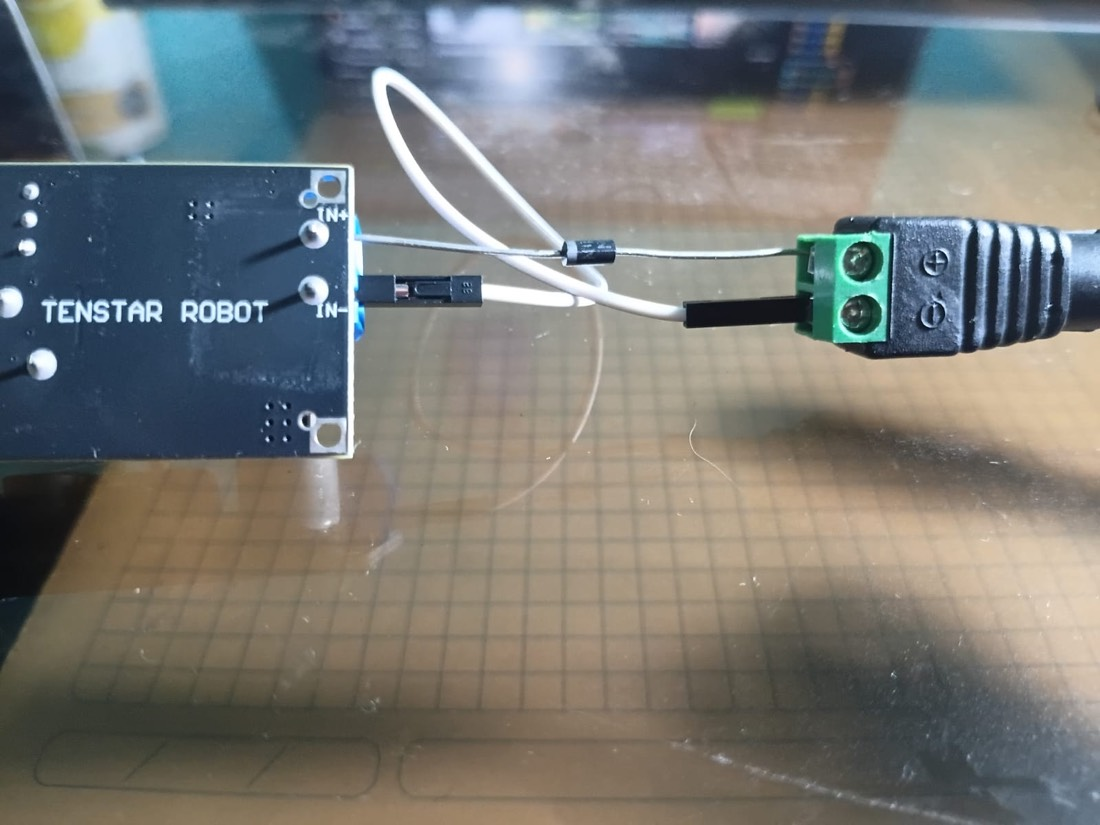
\includegraphics[width=\linewidth]{figuras/v1-conexiones.jpg}}{%
\textbf{Qué se hizo.} Jack DC $\rightarrow$ diodo 1N4007 $\rightarrow$ IN+ del buck y jack $-$ $\rightarrow$ IN$-$, con la salida del buck libre. Sin ESP32 ni código.\\[2pt]
\textbf{Criterio.} El LED del buck enciende; nada se calienta ni huele a quemado.\\[2pt]
\textbf{Resultado.} LED rojo encendido; sin calentamiento. \textbf{Aprobado.}}
\captionof{figure}{V1: plano (izq.) y foto del resultado (der.).}
\end{minipage}

% ---------------------------------------------------------------- V2
\noindent\begin{minipage}{\linewidth}
\vhead{V2}{Fuente: calibrar el buck a 5\,V}{7 nov 2026 · sketch \cod{fuente\_buck}}
\vrow{paso2.jpg}{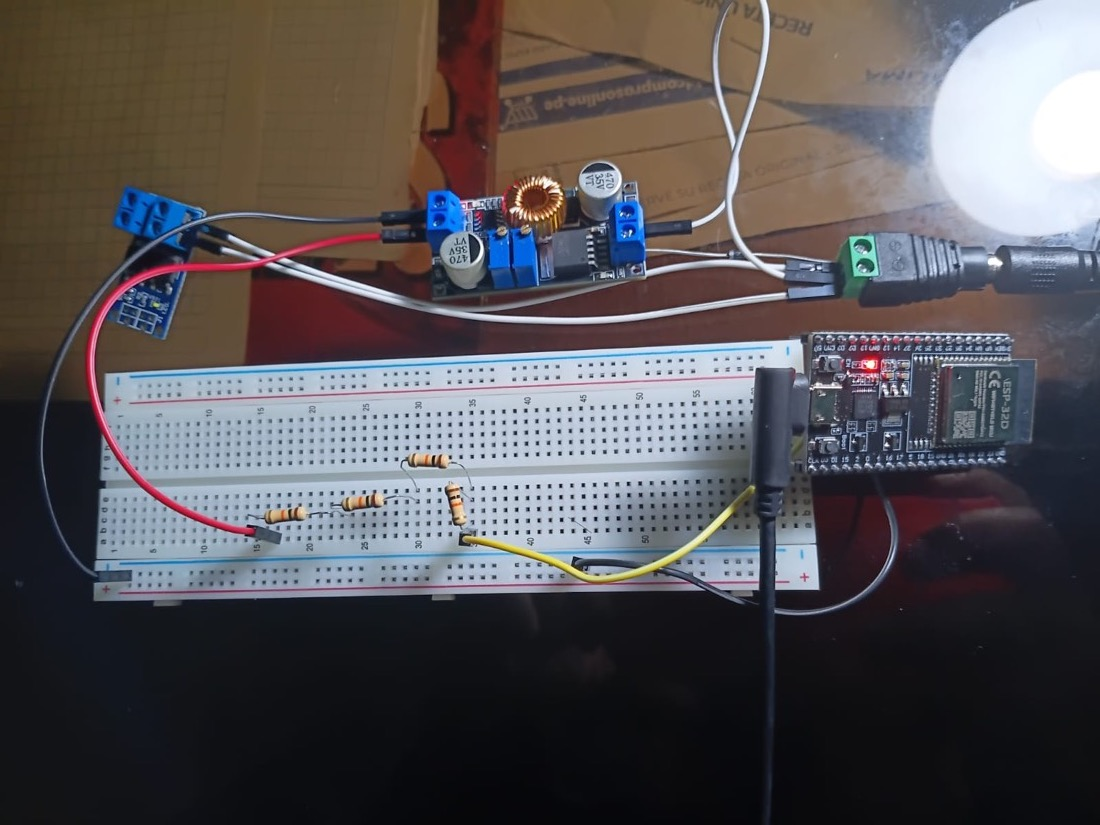
\includegraphics[width=\linewidth]{figuras/v2-armado.jpg}}{%
\textbf{Qué se hizo.} Sin multímetro, el ESP32 midió la salida del buck por D34 a través de un divisor de 4 resistencias de 10\,k$\Omega$ (factor $\times4$). Se giró el tornillo de voltaje hasta ver OK estable.\\[2pt]
\textbf{Criterio.} Entre 4,85 y 5,15\,V con OK de forma estable. Si el programa sube y mide, el ESP32 también queda probado.\\[2pt]
\textbf{Resultado.} De fábrica salía 12,60\,V; quedó en 5,03\,V. \textbf{Aprobado.}}
\begin{minipage}[t]{0.495\linewidth}\begin{Verbatim}[label={\scriptsize\bfseries\ Log esperado\ }]
Prueba - Calibrar el buck a 5 V
Salida del buck: 11.62 V  -> MUY ALTO. NO lo conectes al riel.
Salida del buck:  5.48 V  -> BAJA un poco (gira al otro lado).
Salida del buck:  5.02 V  -> OK, deja el tornillo asi.
\end{Verbatim}
\end{minipage}\hfill
\begin{minipage}[t]{0.495\linewidth}\begin{Verbatim}[label={\scriptsize\bfseries\ Log obtenido\ }]
23:01:34.894 -> Salida del buck: 12.60 V  -> MUY ALTO. ...
...
23:14:58.464 -> Salida del buck: 5.04 V  -> OK, deja el tornillo asi.
23:14:59.181 -> Salida del buck: 5.03 V  -> OK, deja el tornillo asi.
\end{Verbatim}
\end{minipage}
\captionof{figure}{V2: calibración del buck usando el ESP32 como voltímetro.}
\end{minipage}

% ---------------------------------------------------------------- V3
\noindent\begin{minipage}{\linewidth}
\vhead{V3}{Rieles con energía}{8 nov 2026 · sketch \cod{esp32\_vivo}}
\vrow{paso3.jpg}{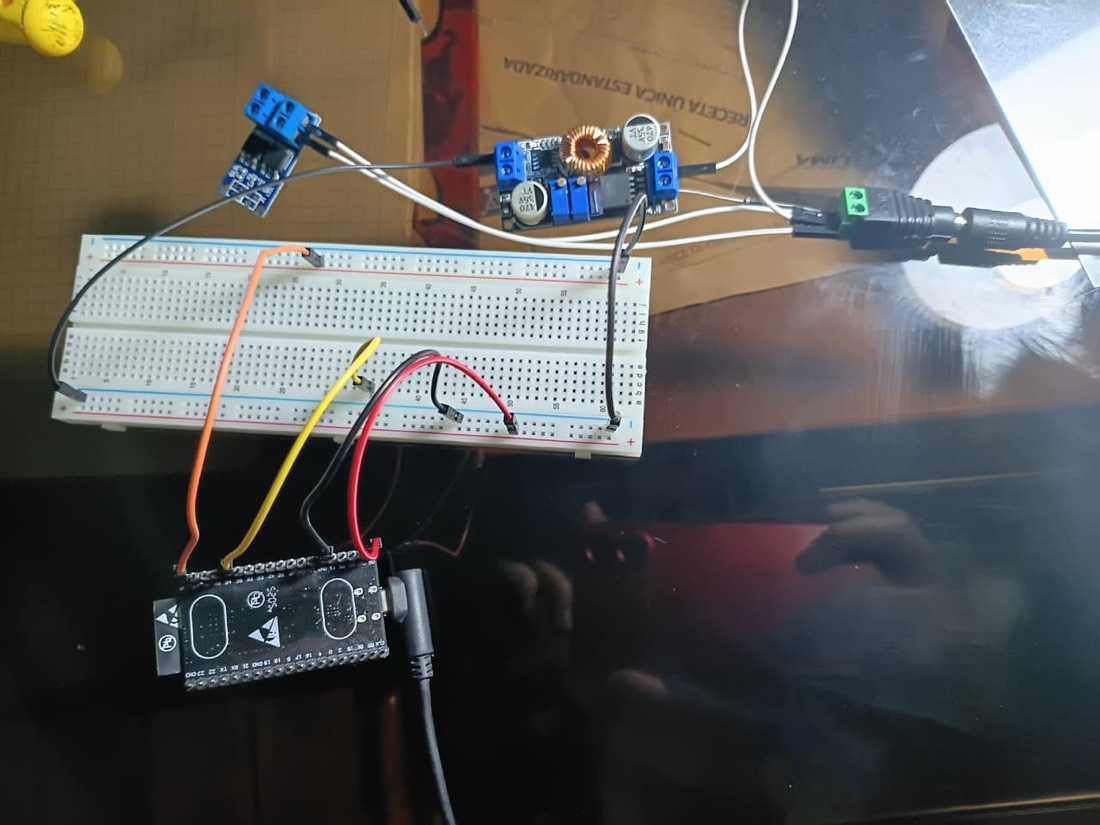
\includegraphics[width=\linewidth]{figuras/v3-rieles.jpg}}{%
\textbf{Qué se hizo.} 5\,V del ESP32 (por USB) al riel + inferior, 3,3\,V al riel + superior y un puente entre los dos rieles de tierra. Se descartan cortos antes de colocar las demás piezas.\\[2pt]
\textbf{Criterio.} El contador supera 60\,s sin volver a 0 (sin reinicios por caída de tensión) y nada se calienta.\\[2pt]
\textbf{Resultado.} Más de 115\,s sin reinicios; ESP32 frío. \textbf{Aprobado.}}
\begin{minipage}[t]{0.495\linewidth}\begin{Verbatim}[label={\scriptsize\bfseries\ Log esperado\ }]
Chip: ESP32-D0WD-V3, 240 MHz
Motivo del ultimo arranque: encendido normal
Vivo 0 s. Si el conteo nunca vuelve a 0, todo bien.
...
Vivo 60 s. Si el conteo nunca vuelve a 0, todo bien.
\end{Verbatim}
\end{minipage}\hfill
\begin{minipage}[t]{0.495\linewidth}\begin{Verbatim}[label={\scriptsize\bfseries\ Log obtenido\ }]
09:07:05.612 -> Vivo 111 s. Si el conteo nunca vuelve a 0, ...
09:07:06.590 -> Vivo 112 s. Si el conteo nunca vuelve a 0, ...
09:07:07.600 -> Vivo 113 s. Si el conteo nunca vuelve a 0, ...
09:07:08.612 -> Vivo 114 s. Si el conteo nunca vuelve a 0, ...
09:07:09.579 -> Vivo 115 s. Si el conteo nunca vuelve a 0, ...
\end{Verbatim}
\end{minipage}
\captionof{figure}{V3: rieles de alimentación y prueba de estabilidad del ESP32.}
\end{minipage}

% ---------------------------------------------------------------- V4
\noindent\begin{minipage}{\linewidth}
\vhead{V4}{LED RGB}{8 nov 2026 · sketch \cod{led\_rgb}}
\vrow{paso4.jpg}{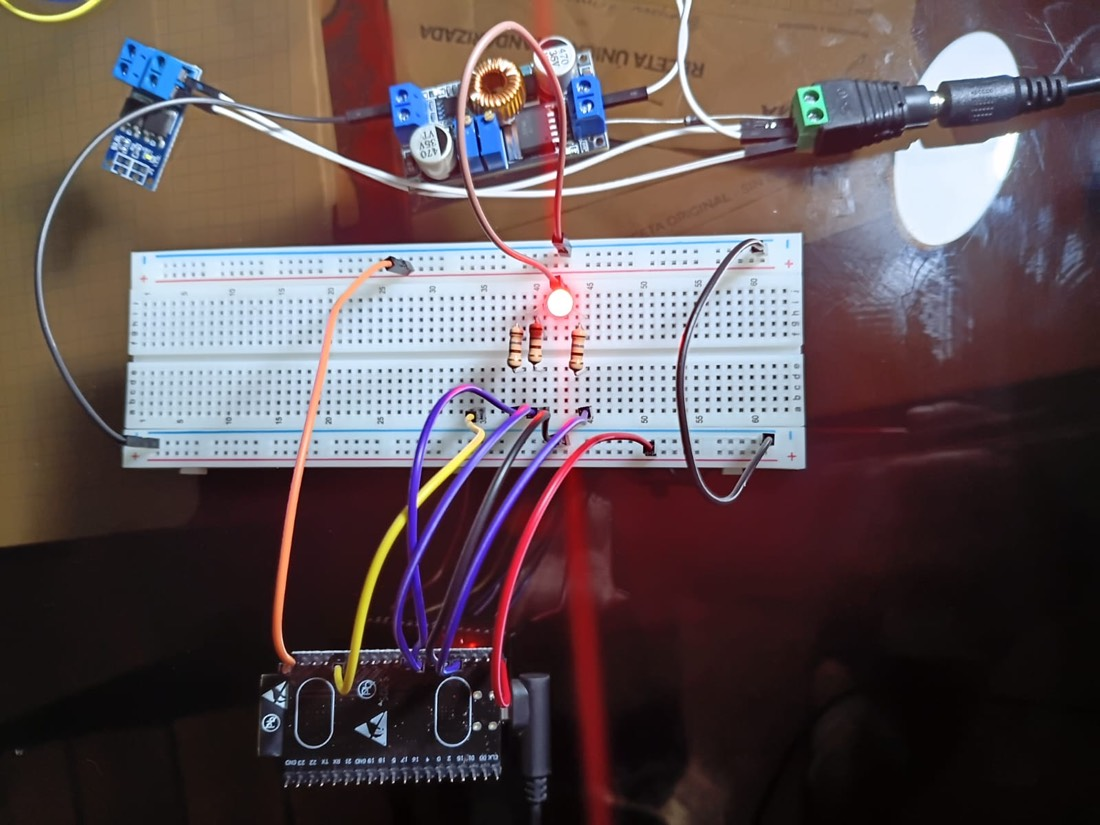
\includegraphics[width=\linewidth]{figuras/v4-led-rgb.jpg}}{%
\textbf{Qué se hizo.} LED RGB de cátodo común con tres resistencias de 180\,$\Omega$ a D13 (R), D14 (G) y D27 (B). El programa recorre los colores e imprime el que debería verse.\\[2pt]
\textbf{Criterio.} Cada color coincide con el mensaje y en APAGADO no hay luz.\\[2pt]
\textbf{Resultado.} Los cuatro estados coinciden; también queda probado el puente de tierra de V3. \textbf{Aprobado.}}
\begin{minipage}[t]{0.495\linewidth}\begin{Verbatim}[label={\scriptsize\bfseries\ Log esperado\ }]
Prueba - LED RGB
El LED debe mostrar el color que se imprime.
Ahora: ROJO
Ahora: VERDE
Ahora: AZUL
Ahora: APAGADO
\end{Verbatim}
\end{minipage}\hfill
\begin{minipage}[t]{0.495\linewidth}\begin{Verbatim}[label={\scriptsize\bfseries\ Log obtenido\ }]
09:42:44.050 -> Ahora: ROJO
09:42:45.557 -> Ahora: VERDE
09:42:47.064 -> Ahora: AZUL
09:42:48.550 -> Ahora: APAGADO
09:42:50.065 -> Ahora: ROJO
\end{Verbatim}
\end{minipage}
\captionof{figure}{V4: LED RGB de estado.}
\end{minipage}

% ---------------------------------------------------------------- V5
\noindent\begin{minipage}{\linewidth}
\vhead{V5}{Buzzer}{8 nov 2026 · sketch \cod{buzzer}}
\vrow{paso5.jpg}{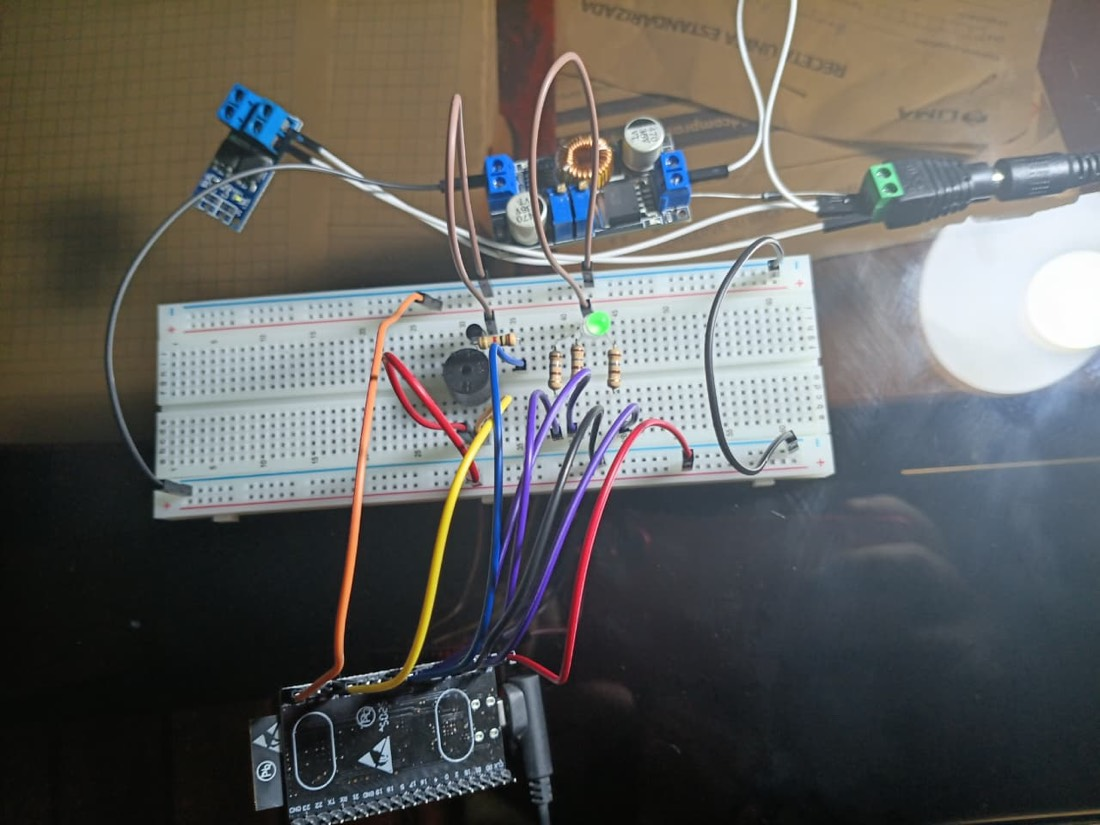
\includegraphics[width=\linewidth]{figuras/v5-buzzer.jpg}}{%
\textbf{Qué se hizo.} Buzzer activo de 5\,V conmutado por un 2N2222, con la base a D26 por 1\,k$\Omega$: el ESP32 no alimenta el buzzer directamente.\\[2pt]
\textbf{Criterio.} Suenan 3 pitidos cada vez que aparece ``Pitando...''.\\[2pt]
\textbf{Resultado.} 3 pitidos por mensaje, cada $\approx$\,6\,s. \textbf{Aprobado.}}
\begin{minipage}[t]{0.495\linewidth}\begin{Verbatim}[label={\scriptsize\bfseries\ Log esperado\ }]
Prueba - Buzzer
Deben sonar 3 pitidos cortos cada 5 s.
Pitando...
Pitando...
\end{Verbatim}
\end{minipage}\hfill
\begin{minipage}[t]{0.495\linewidth}\begin{Verbatim}[label={\scriptsize\bfseries\ Log obtenido\ }]
10:02:11.815 -> Pitando...
10:02:17.700 -> Pitando...
10:02:23.609 -> Pitando...
10:02:29.530 -> Pitando...
\end{Verbatim}
\end{minipage}
\captionof{figure}{V5: alarma sonora con transistor.}
\end{minipage}

% ---------------------------------------------------------------- V6
\noindent\begin{minipage}{\linewidth}
\vhead{V6}{DHT22: temperatura y humedad}{8 nov 2026 · sketch \cod{dht22}}
\vrow{paso6.jpg}{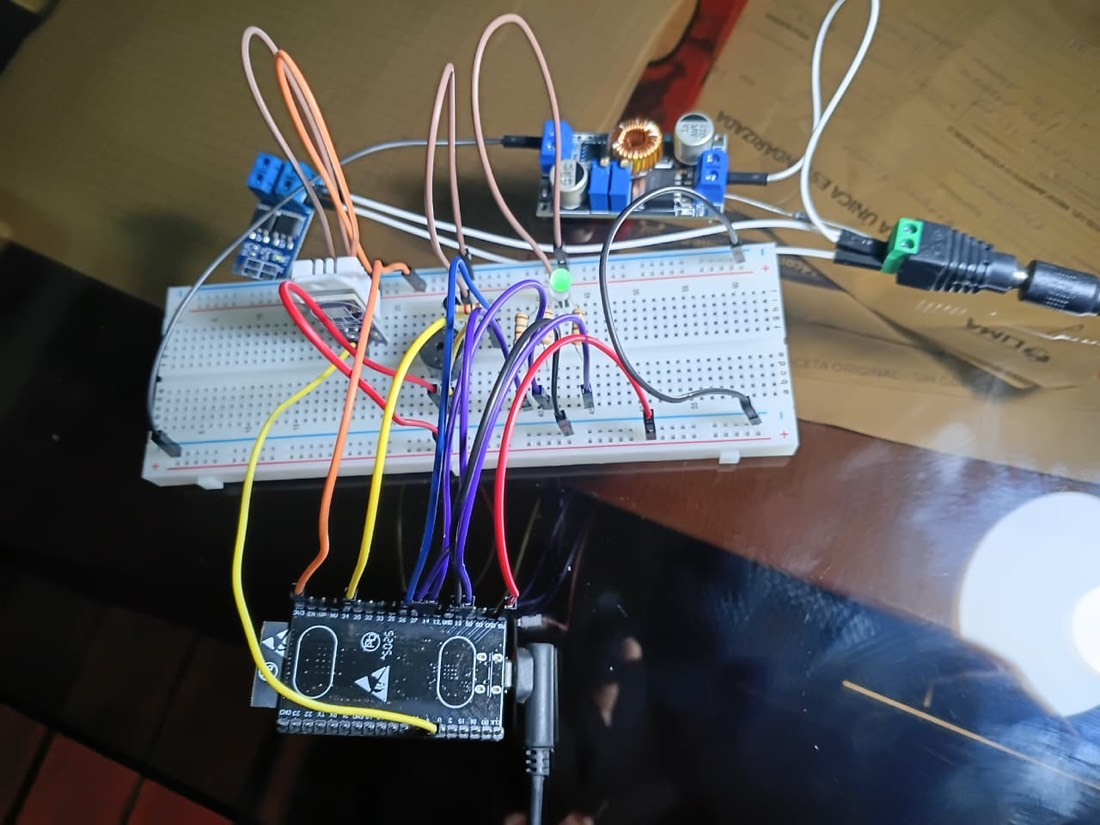
\includegraphics[width=\linewidth]{figuras/v6-dht22.jpg}\\[2pt]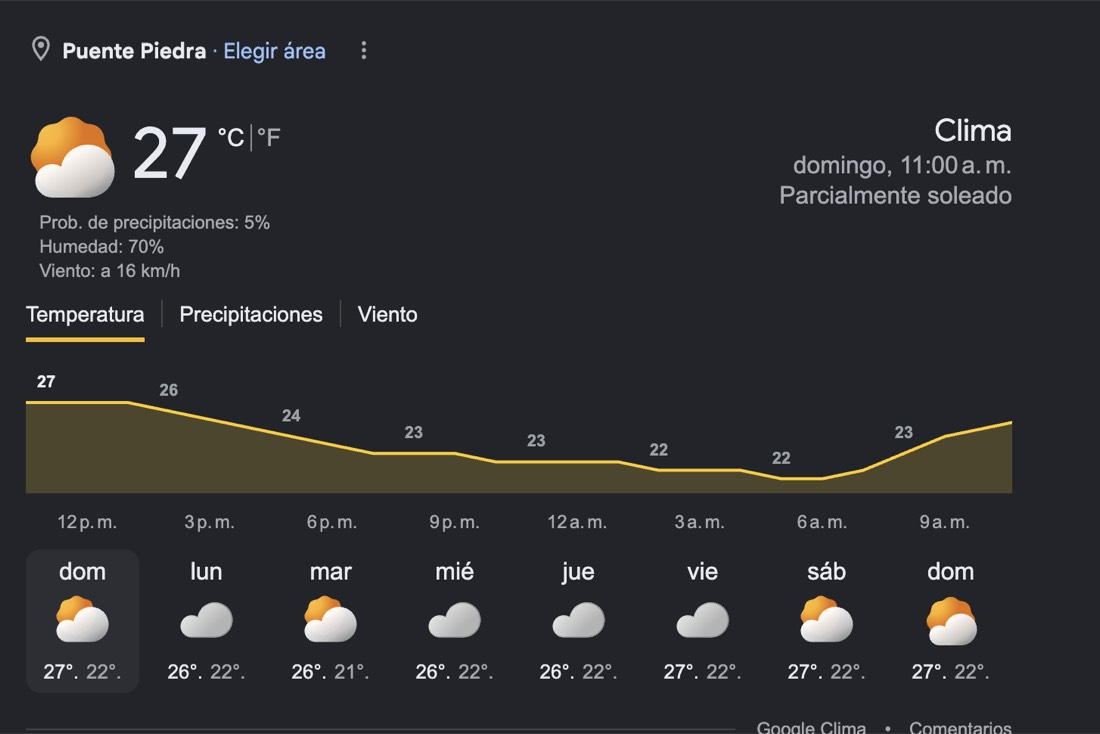
\includegraphics[width=0.85\linewidth]{figuras/v6-clima.jpg}}{%
\textbf{Qué se hizo.} DHT22 a 3,3\,V con datos en D4. Se comparó con la referencia meteorológica de la hora (abajo) y se sopló cerca para ver la respuesta de la humedad.\\[2pt]
\textbf{Criterio.} Dice OK con la temperatura del cuarto y la humedad sube al soplar.\\[2pt]
\textbf{Resultado.} 27,7\,$^\circ$C y 74\,\% frente a 27\,$^\circ$C y 70\,\% de la referencia; al soplar, 74 $\rightarrow$ 84\,\% y regresa sola. Un primer montaje invertido calentó el sensor (31,8\,$^\circ$C) y se corrigió. \textbf{Aprobado.}}
\begin{minipage}[t]{0.495\linewidth}\begin{Verbatim}[label={\scriptsize\bfseries\ Log esperado\ }]
Prueba - DHT22
OK: 24.3 C, 58 % de humedad. Sopla cerca y la humedad debe subir.
OK: 24.6 C, 71 % de humedad. Sopla cerca y la humedad debe subir.
\end{Verbatim}
\end{minipage}\hfill
\begin{minipage}[t]{0.495\linewidth}\begin{Verbatim}[label={\scriptsize\bfseries\ Log obtenido\ }]
11:30:56.153 -> OK: 27.7 C, 74 % de humedad. ...
11:31:03.636 -> OK: 27.8 C, 80 % de humedad. ...
11:31:08.676 -> OK: 27.8 C, 84 % de humedad. ...
11:31:21.180 -> OK: 27.9 C, 77 % de humedad. ...
\end{Verbatim}
\end{minipage}
\captionof{figure}{V6: DHT22 contrastado con la referencia meteorológica.}
\end{minipage}

% ---------------------------------------------------------------- V7
\noindent\begin{minipage}{\linewidth}
\vhead{V7}{Sensores MQ-135 y MQ-7}{8 nov 2026 · sketch \cod{sensores\_mq}}
\vrow{paso7.jpg}{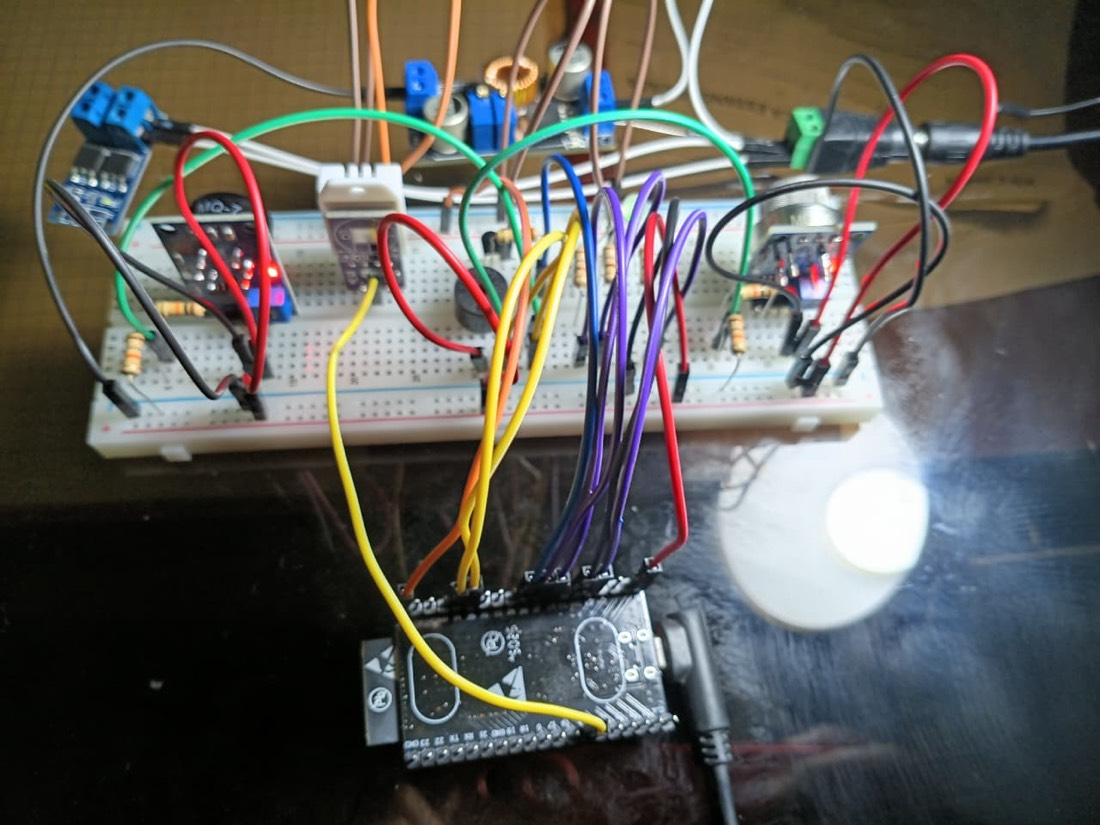
\includegraphics[width=\linewidth]{figuras/v7-sensores-mq.jpg}}{%
\textbf{Qué se hizo.} MQ-135 (D34) y MQ-7 (D35) a 5\,V, cada uno con un divisor 10\,k$\Omega$/18\,k$\Omega$ para que su salida no supere 3,3\,V en el ADC. Tras 2--3\,min de precalentamiento se sopló sobre el MQ-135.\\[2pt]
\textbf{Criterio.} Ambos dicen OK (pin $<$ 3,3\,V) y el MQ-135 sube al soplar.\\[2pt]
\textbf{Resultado.} MQ-135: 0,38 $\rightarrow$ 0,46\,V al soplar y vuelve; MQ-7 estable en 1,09\,V. \textbf{Aprobado.}}
\begin{minipage}[t]{0.495\linewidth}\begin{Verbatim}[label={\scriptsize\bfseries\ Log esperado\ }]
Prueba - Sensores MQ
Los MQ necesitan 2-3 minutos para calentarse.
MQ-135  pin  612 mV  (sensor 0.95 V)  OK
MQ-7    pin  398 mV  (sensor 0.62 V)  OK
MQ-135  pin  981 mV  (sensor 1.53 V)  OK
\end{Verbatim}
\end{minipage}\hfill
\begin{minipage}[t]{0.495\linewidth}\begin{Verbatim}[label={\scriptsize\bfseries\ Log obtenido\ }]
13:07:58.975 -> MQ-135  pin  247 mV  (sensor 0.38 V)  OK
13:07:59.188 -> MQ-7    pin  705 mV  (sensor 1.10 V)  OK
13:08:01.391 -> MQ-135  pin  296 mV  (sensor 0.46 V)  OK
13:08:01.607 -> MQ-7    pin  702 mV  (sensor 1.09 V)  OK
13:08:13.391 -> MQ-135  pin  226 mV  (sensor 0.35 V)  OK
\end{Verbatim}
\end{minipage}
\captionof{figure}{V7: sensores de gas con sus divisores de tensión.}
\end{minipage}

% ---------------------------------------------------------------- V8
\noindent\begin{minipage}{\linewidth}
\vhead{V8}{Nodo sin laptop}{8 nov 2026 · multímetro Truper MUT-830}
\vrow{paso8.jpg}{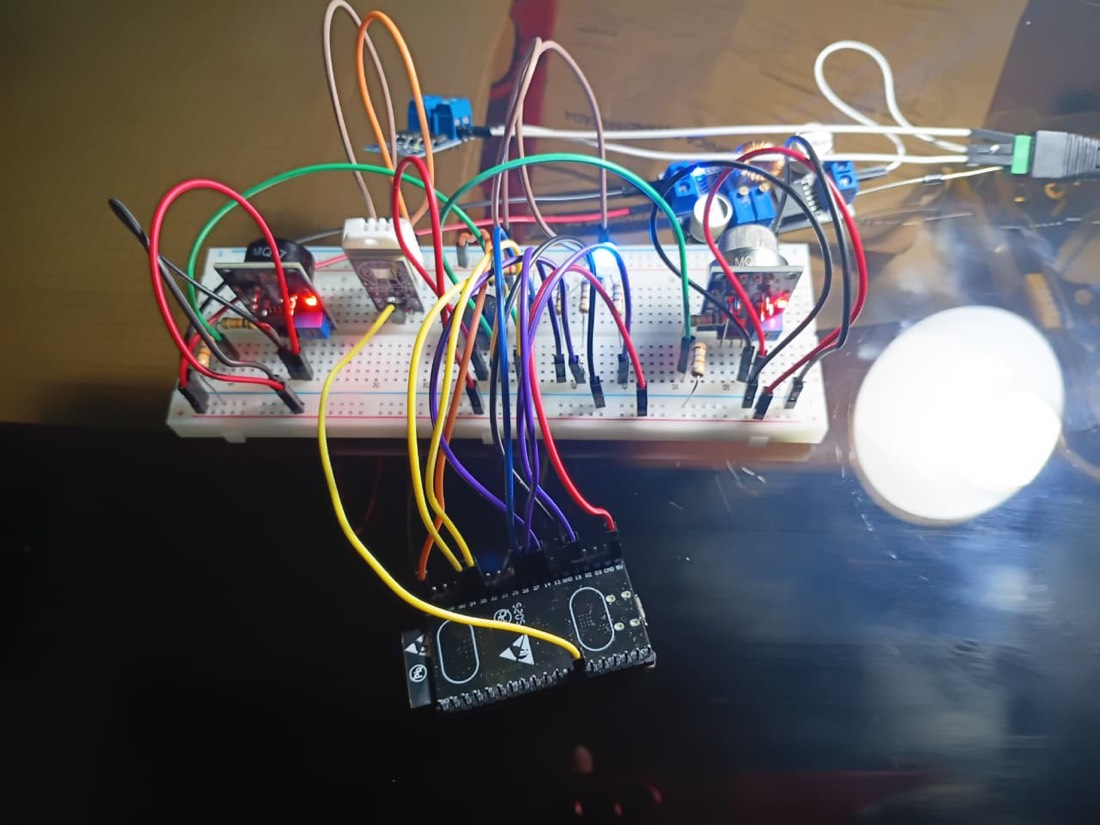
\includegraphics[width=\linewidth]{figuras/v8-sin-laptop.jpg}}{%
\textbf{Qué se hizo.} OUT+ del buck al riel de 5\,V y USB desconectado: el nodo se alimenta solo de los 12\,V. Con multímetro se fijó el voltaje en vacío y el límite de corriente del buck.\\[2pt]
\textbf{Criterio.} 4,95--5,10\,V en vacío; límite de 1,20\,A ($\approx$\,2× el consumo del nodo); el LED recorre sus colores sin reinicios.\\[2pt]
\textbf{Resultado.} Falla inicial detectada y corregida (abajo). \textbf{Aprobado.}}
\begin{minipage}[t]{0.495\linewidth}\begin{Verbatim}[label={\scriptsize\bfseries\ Mediciones esperadas\ }]
Vacio (OUT+ al aire), DCV 20 ......... 4.95 - 5.10 V
Limite de corriente, 10ADC ........... 1.20 A
Con carga (OUT+ en el riel) .......... ~5.0 V
OUT+ a GND sin energia, Ohm 200 ...... ~17 Ohm (MQ), no ~0
\end{Verbatim}
\end{minipage}\hfill
\begin{minipage}[t]{0.495\linewidth}\begin{Verbatim}[label={\scriptsize\bfseries\ Mediciones obtenidas\ }]
Inicio: nada enciende; vacio = 1.25 V   -> FALLA
  causa: limite de corriente al minimo (tope de V2)
OUT+ a GND ........................... 17.5 Ohm (sin corto)
Tras reajuste: vacio ................. 5.0 V
Limite fijado ........................ 1.2 A
Con carga: ESP32, MQ y LED funcionan . OK
\end{Verbatim}
\end{minipage}
\captionof{figure}{V8: nodo autónomo; la falla del límite de corriente solo se detectó al quitar el USB.}
\end{minipage}

% ---------------------------------------------------------------- V9
\noindent\begin{minipage}{\linewidth}
\vhead{V9}{Ventilador de 12\,V por el HW-517}{13 nov 2026 · sketch \cod{ventilador}}
\vrow{paso9.jpg}{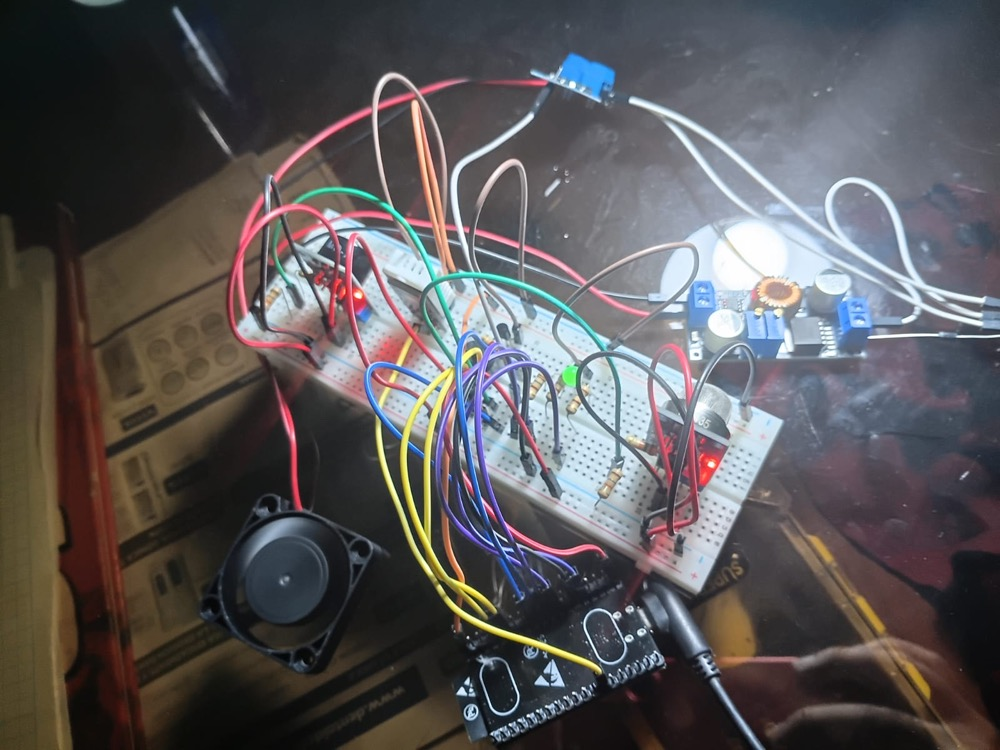
\includegraphics[width=\linewidth]{figuras/v9-ventilador.jpg}}{%
\textbf{Qué se hizo.} El ventilador disponible es de 2 cables (sin tacómetro), así que no admite PWM directo: se conectó a OUT+/OUT$-$ del módulo HW-517 y el ESP32 envía PWM por D25 a su entrada TRIG. El programa recorre 0, 40, 60, 80 y 100\,\%.\\[2pt]
\textbf{Criterio.} Parado en 0\,\% y velocidad creciente, visible y audible, hasta el 100\,\%.\\[2pt]
\textbf{Resultado.} A 25\,kHz solo giraba al 100\,\%: el optoacoplador del HW-517 no conmuta a esa frecuencia. Con 100\,Hz arranca desde el 40\,\% y acelera de forma gradual. El firmware del nodo se ajustó a 100\,Hz. \textbf{Aprobado.}}
\begin{minipage}[t]{0.495\linewidth}
\begin{Verbatim}[label={\scriptsize\bfseries\ Log esperado\ }]
Prueba - Ventilador (2 cables, HW-517)
PWM   0 %  ->  debe estar PARADO
PWM  40 %  ->  gira lento (puede no arrancar)
PWM  60 %  ->  gira mas rapido que el paso anterior
PWM 100 %  ->  a fondo
\end{Verbatim}
\end{minipage}\hfill
\begin{minipage}[t]{0.495\linewidth}
\begin{Verbatim}[label={\scriptsize\bfseries\ Log obtenido (100 Hz)\ }]
15:39:37.055 -> PWM   0 %  ->  debe estar PARADO
15:39:42.047 -> PWM  40 %  ->  gira lento (...)
15:39:47.049 -> PWM  60 %  ->  gira mas rapido (...)
15:39:52.048 -> PWM  80 %  ->  gira mas rapido (...)
15:39:57.046 -> PWM 100 %  ->  a fondo
\end{Verbatim}
\end{minipage}
\captionof{figure}{V9: control de velocidad del ventilador a través del HW-517.}
\end{minipage}

% ---------------------------------------------------------------- V10
\noindent\begin{minipage}{\linewidth}
\vhead{V10}{Integración: firmware completo y nube}{desde 9 nov 2026 · \cod{nodo.ino}}
\vrow{paso10.jpg}{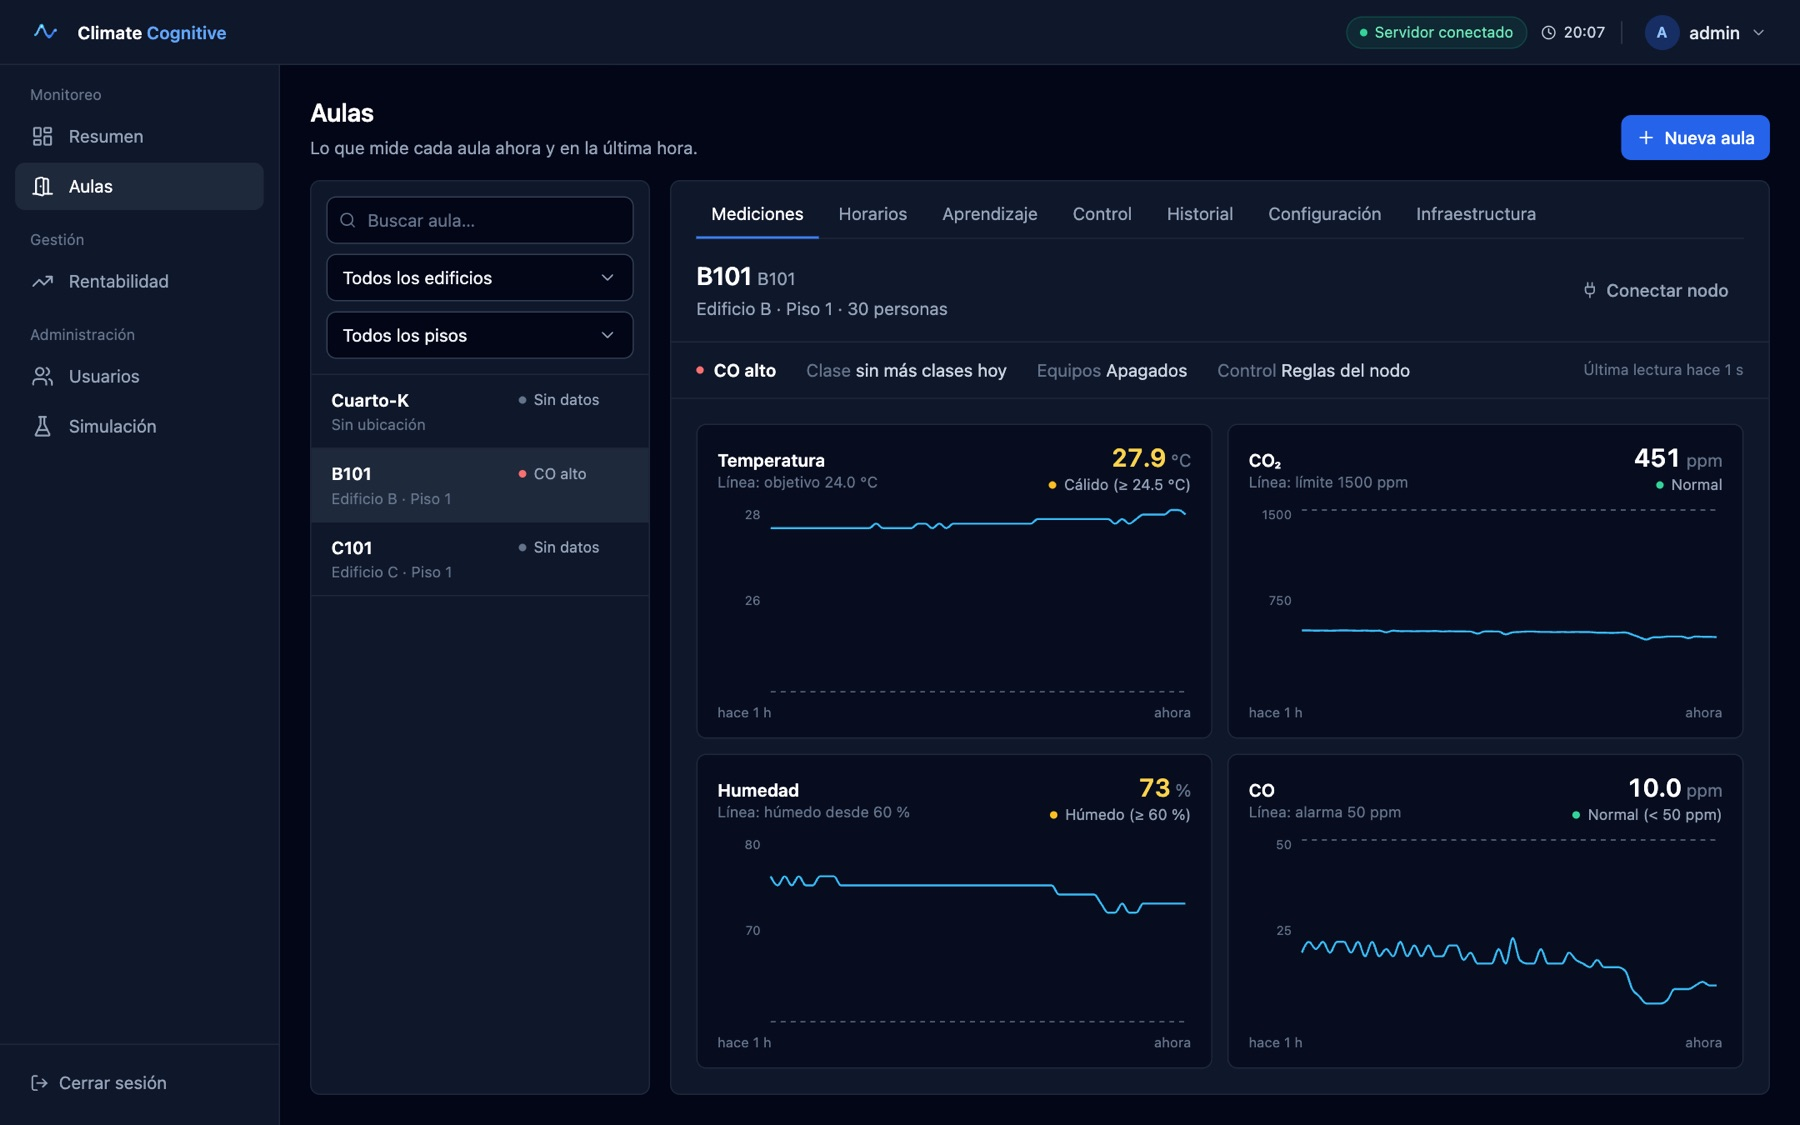
\includegraphics[width=\linewidth]{figuras/dash-mediciones.jpg}}{%
\textbf{Qué se hizo.} Se cargó el firmware completo (reglas, histéresis, alarma de CO, MQTT/TLS); la conexión a la nube se verificó antes de tener el ventilador. El nodo publica a la VM en la nube y el \emph{dashboard} muestra sus lecturas (der.).\\[2pt]
\textbf{Criterio.} Conecta a WiFi y al broker, emite un bloque CICLO por lectura, el estado sigue las reglas y el \emph{dashboard} muestra los mismos valores que el monitor serie.\\[2pt]
\textbf{Resultado.} Conexión y telemetría verificadas; B101 opera sin interrupciones desde el 9 nov. Con el umbral inicial (300) el aula queda \emph{vacía} y el estado en Desactivado (Hallazgo~1). Las reglas de enfriamiento, intervalo mínimo y alarma de CO se están validando con el ventilador ya conectado (V9) y el umbral recalibrado. \textbf{Aprobado con observación.}}
\captionof{figure}{V10: el nodo integrado publicando a la plataforma.}
\end{minipage}

\subsection{Versión en PCB: hacia el producto final}
\label{sec:pcb}
El protoboard sirvió para validar cada bloque por separado, pero no es instalable en un aula: los cables se sueltan, ocupa espacio y no protege los circuitos. Por eso el equipo diseñó en KiCad una placa de circuito impreso que reúne todo el nodo y que representa lo más cercano a la versión final del producto. La placa se fabricó a través de un contacto del profesor del curso a partir de los archivos Gerber generados en KiCad. El esquemático (Fig.~\ref{fig:pcb-esq}) agrupa el circuito en cinco bloques: alimentación de 12 a 5\,V con medición de corriente, controlador ESP32, sensores, actuador de 12\,V y alarma de CO.

\begin{figure}[H]
\centering
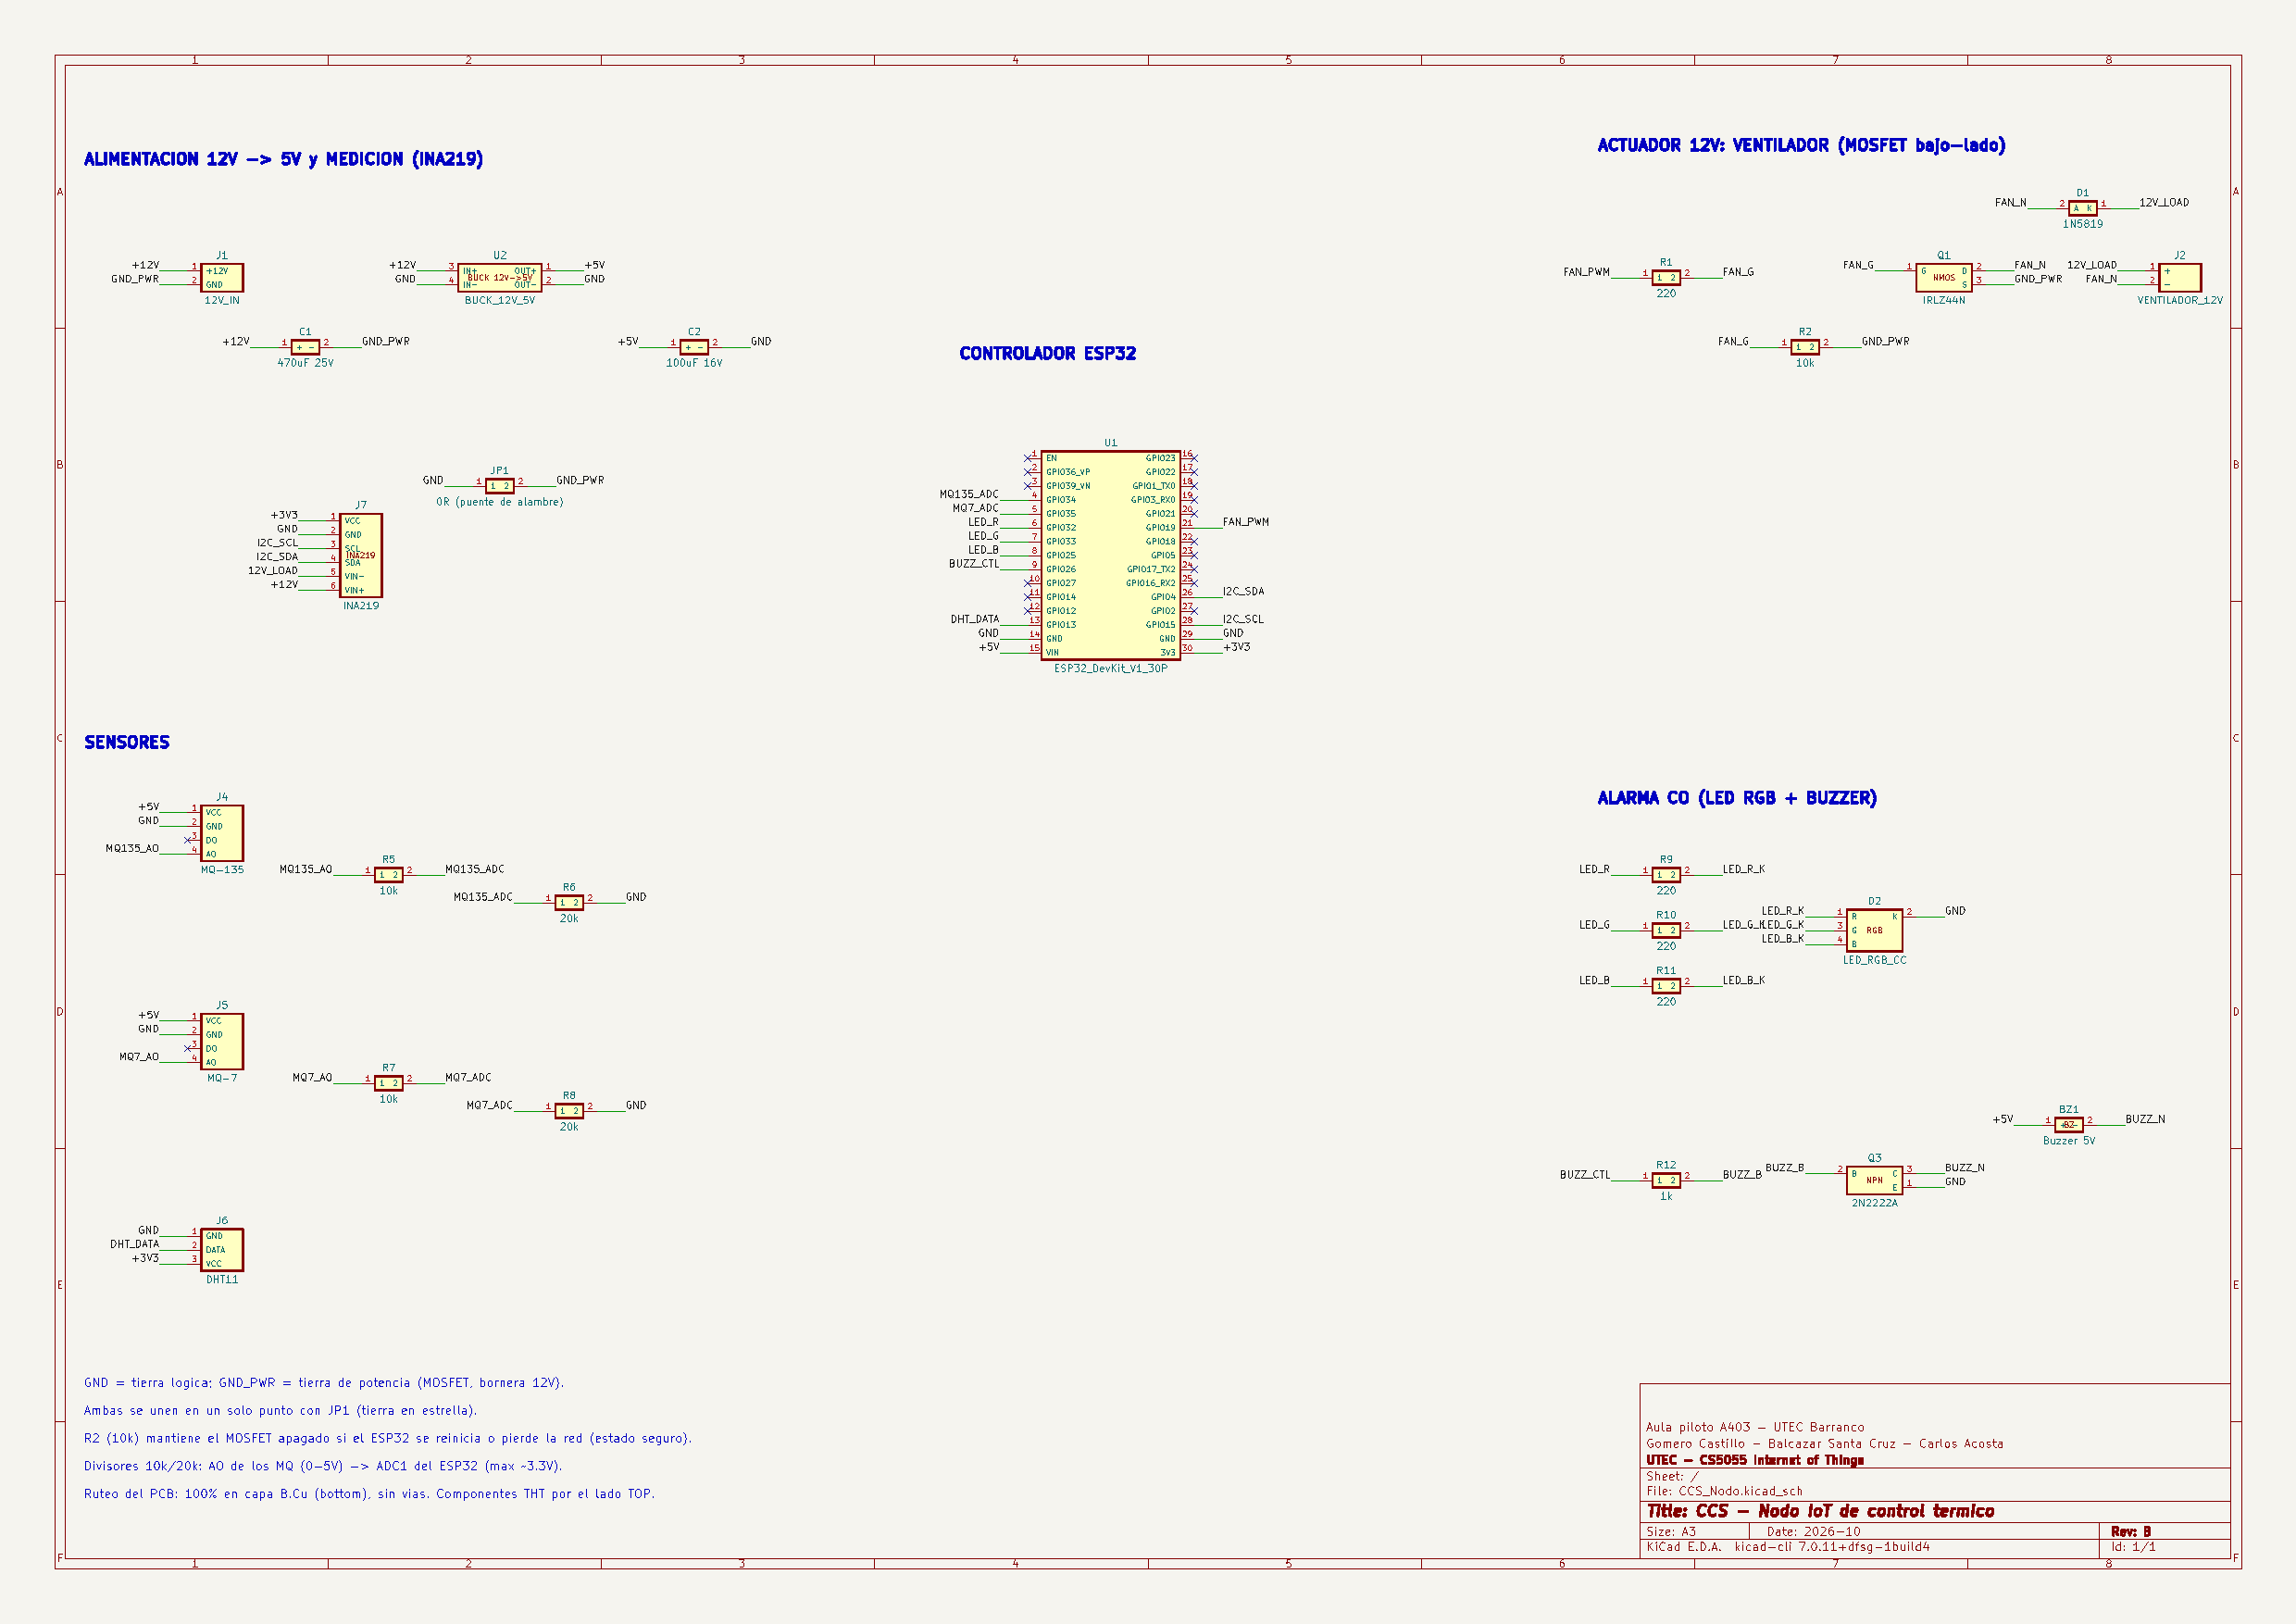
\includegraphics[width=\linewidth,trim={30 60 30 30},clip]{figuras/pcb-esquematico.pdf}
\caption{Esquemático del nodo en KiCad, elaborado por el equipo.}
\label{fig:pcb-esq}
\end{figure}

\textbf{Decisiones de diseño.} La placa mide 100\,×\,84\,mm, con componentes de inserción (THT) para poder soldarla a mano. Además de las reglas pedidas por el curso, se tomaron las siguientes decisiones:
\begin{itemize}[leftmargin=12pt]
  \item \textbf{Ruteo en una sola cara.} Todas las pistas van en la cara inferior, sin vías y con quiebres a 45°.
  \item \textbf{Ancho de pista según la corriente.} 2,0\,mm para los 12\,V y el ventilador, 1,2\,mm para 5\,V, 1,0\,mm para tierra, 0,8\,mm para 3,3\,V y 0,6\,mm para señales.
  \item \textbf{Tierras separadas.} El retorno de potencia (GND\_PWR: MOSFET y bornera de 12\,V) y la tierra lógica (GND) son planos distintos que se unen en un solo punto, el puente JP1 (tierra en estrella). Así el ruido del ventilador no afecta las lecturas analógicas de los MQ.
  \item \textbf{Antena libre.} Bajo la antena del ESP32 no hay cobre y la antena queda en el borde de la placa, para no degradar el WiFi.
  \item \textbf{Ventilador por MOSFET de lado bajo.} Un IRLZ44N de nivel lógico, con diodo 1N5819 de rueda libre. R2 (10\,k$\Omega$) mantiene el MOSFET apagado si el ESP32 se reinicia (estado seguro).
  \item \textbf{Medición de consumo.} La PCB integra un INA219 en el circuito del ventilador, conectado por I$^2$C a GPIO4/15. El nodo lee tensión, corriente y potencia; estas mediciones permiten calcular la energía consumida, en lugar de inferirla únicamente del nivel de PWM.
  \item \textbf{Divisores 10\,k$\Omega$/20\,k$\Omega$ en los MQ.} Su salida de 0--5\,V queda dentro del ADC de 3,3\,V.
  \item \textbf{Reutilización de módulos.} En el ensamblado se usaron el mismo módulo MOSFET (HW-517) y el mismo buck (XL4015) del protoboard, de modo que la placa no requirió comprar otros actuadores ni otra fuente.
  \item \textbf{Calefactor fuera de esta versión.} Su bloque se retiró y GPIO18 queda reservado para incorporarlo después.
\end{itemize}

\begin{figure}[H]
\centering
\begin{subfigure}[t]{0.495\linewidth}\centering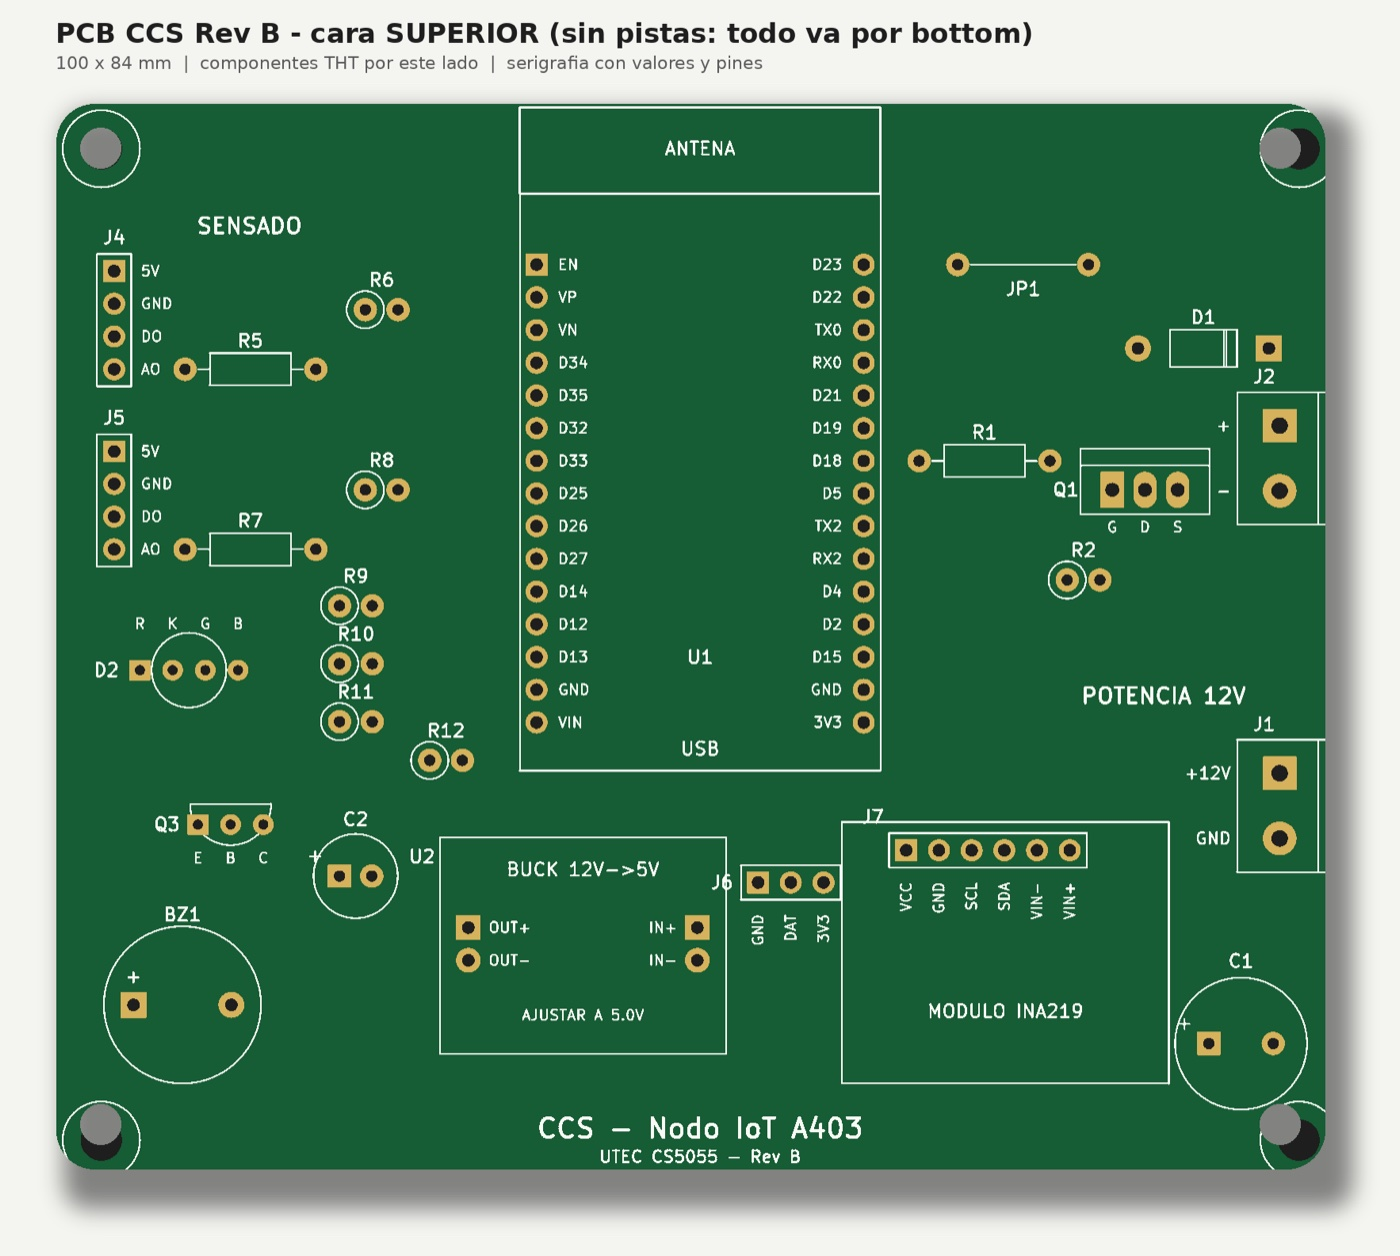
\includegraphics[width=\linewidth]{figuras/pcb-superior.jpg}\caption{Cara superior: componentes y serigrafía.}\end{subfigure}\hfill
\begin{subfigure}[t]{0.495\linewidth}\centering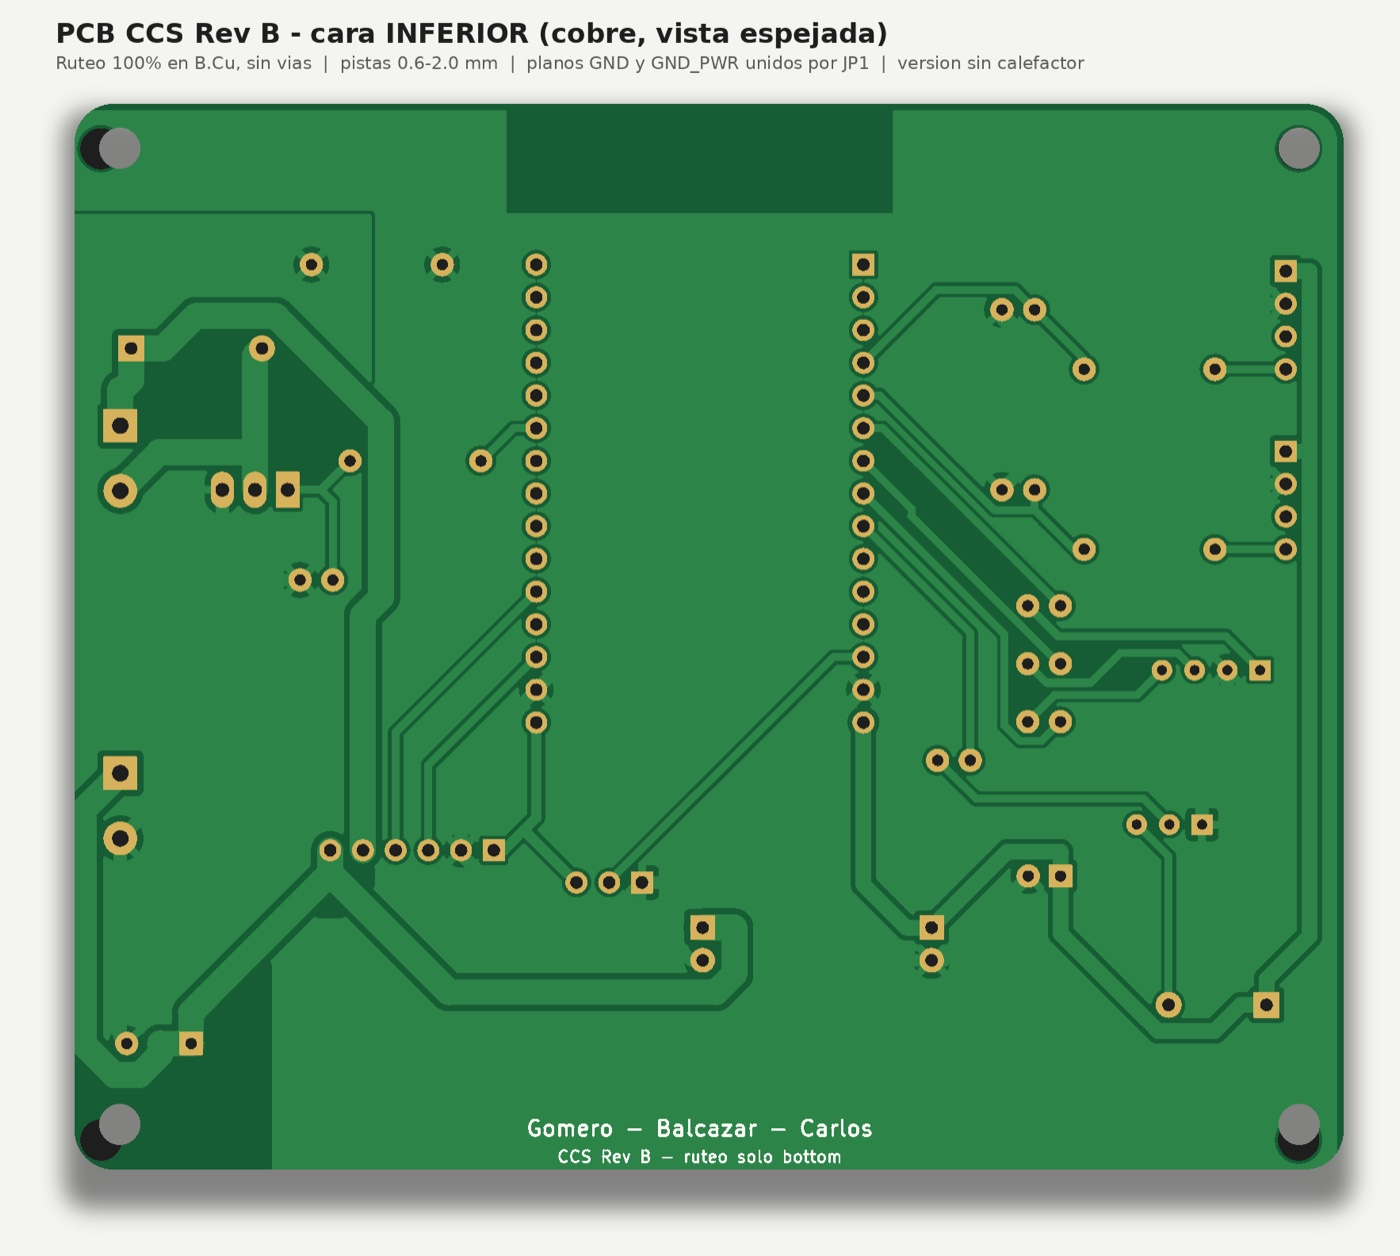
\includegraphics[width=\linewidth]{figuras/pcb-inferior.jpg}\caption{Cara inferior: todo el ruteo, con planos GND y GND\_PWR.}\end{subfigure}
\caption{Diseño del PCB en KiCad.}
\label{fig:pcb-layout}
\end{figure}

\begin{figure}[H]
\centering
\begin{subfigure}[t]{0.40\linewidth}\centering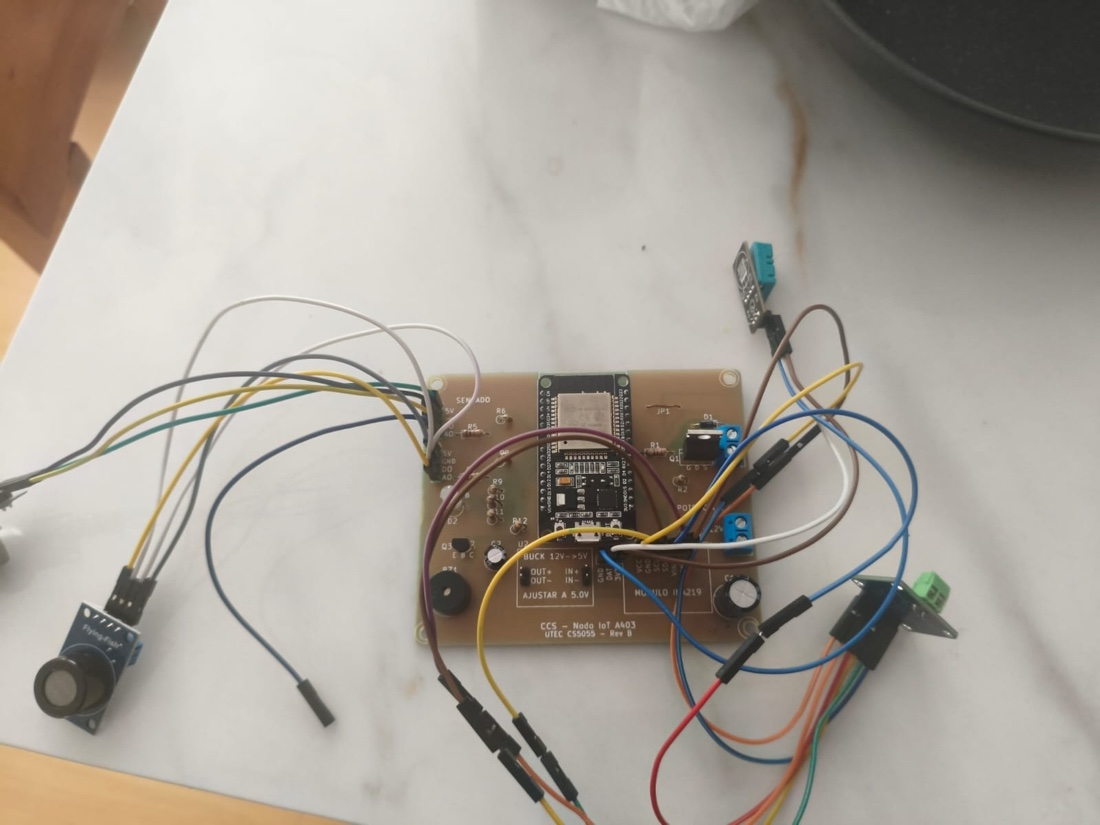
\includegraphics[width=\linewidth]{figuras/pcb-foto-top.jpg}\caption{Placa fabricada y ensamblada: ESP32, buck, borneras de 12\,V y del ventilador, y MQ y DHT11 por cable en la zona de sensado.}\end{subfigure}\hfill
\begin{subfigure}[t]{0.40\linewidth}\centering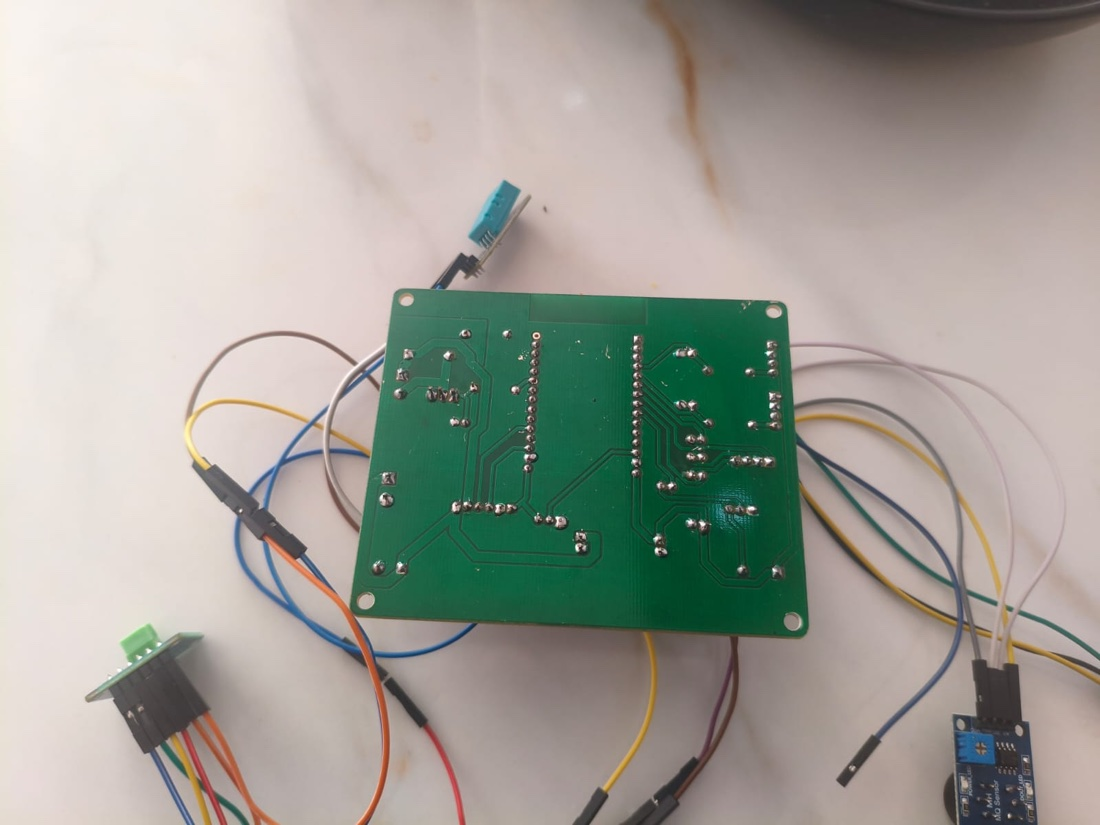
\includegraphics[width=\linewidth]{figuras/pcb-foto-bottom.jpg}\caption{Cara inferior soldada: coincide con el ruteo de la Fig.~\ref{fig:pcb-layout}b.}\end{subfigure}
\caption{Evidencia física de la PCB fabricada.}
\label{fig:pcb-fotos}
\end{figure}

\begin{figure}[H]
\centering
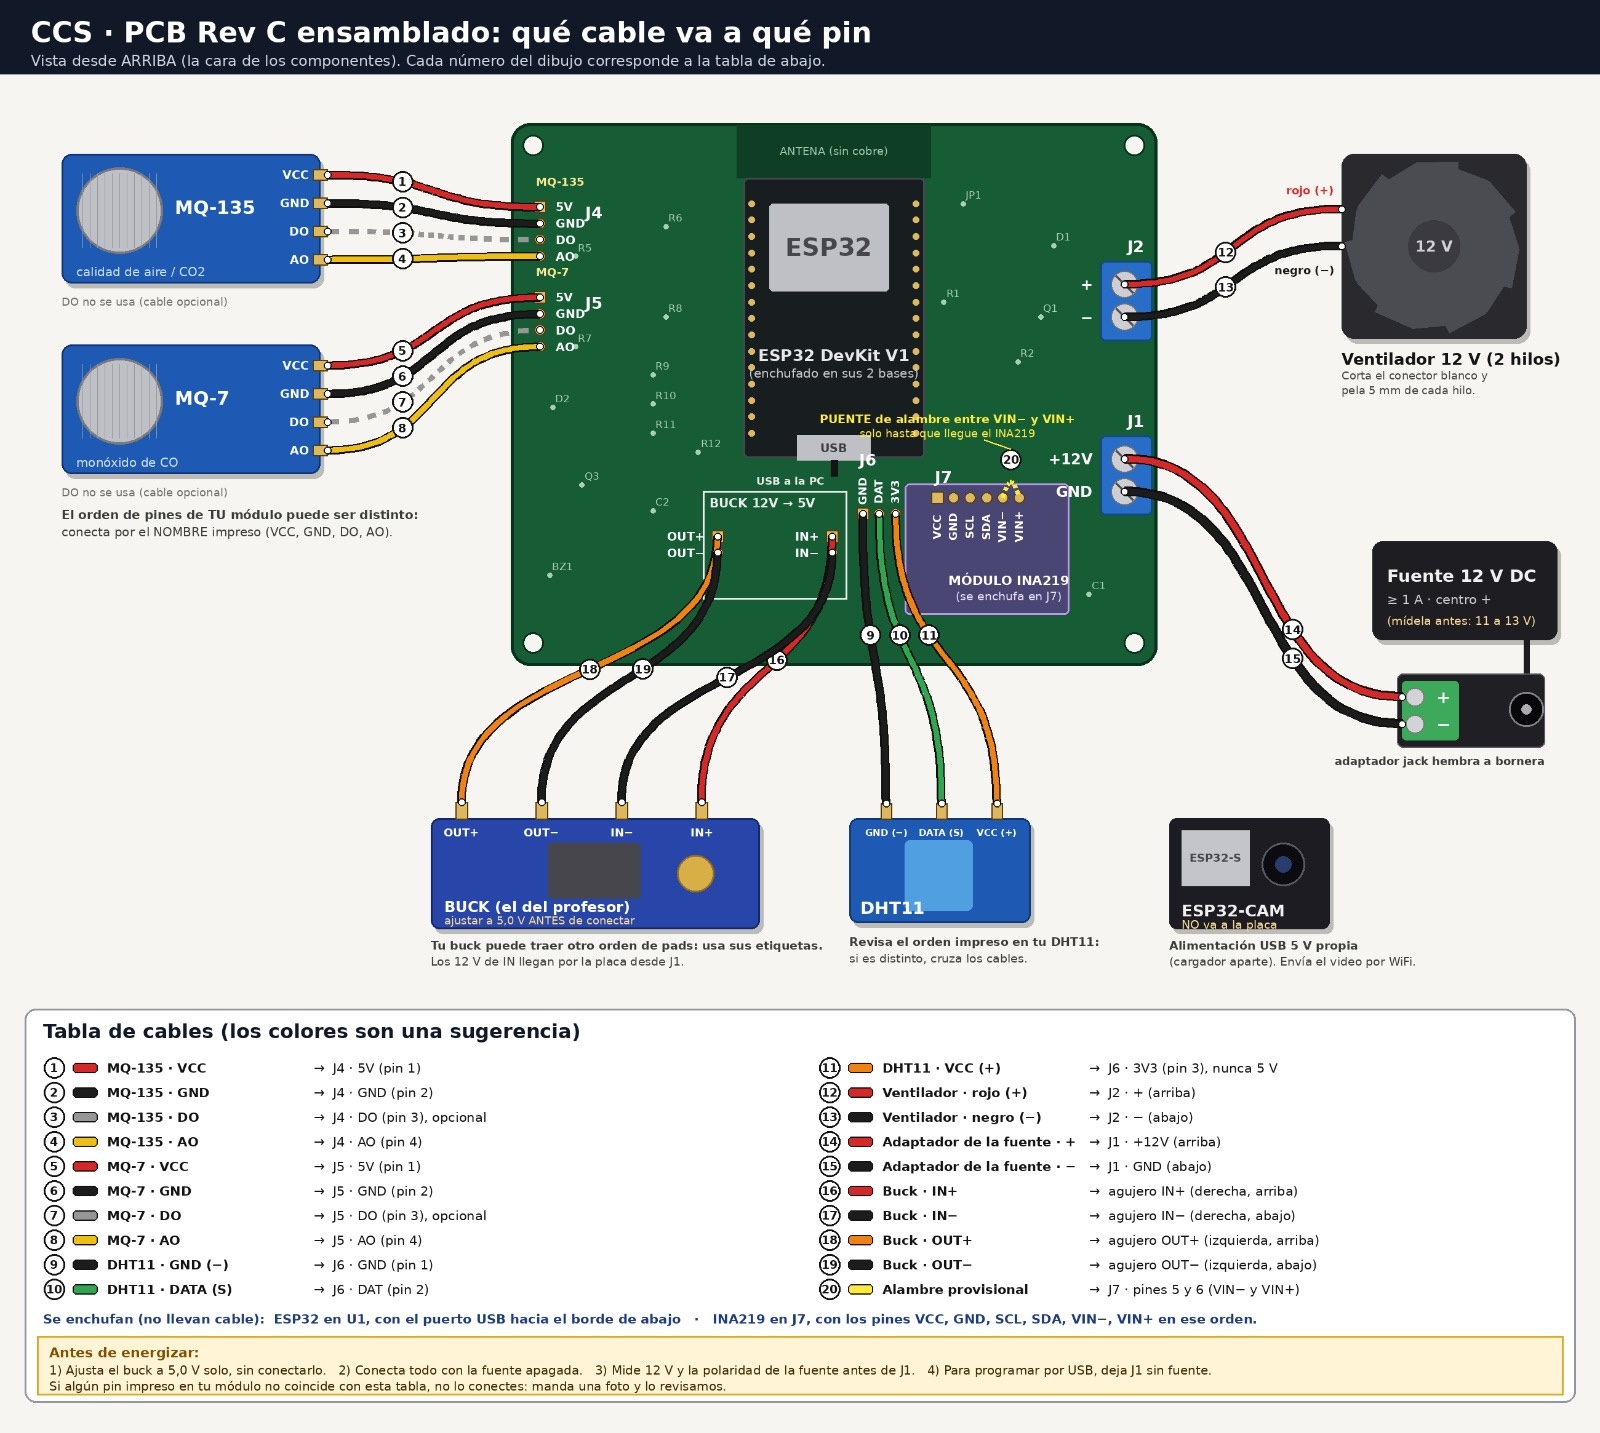
\includegraphics[width=0.85\linewidth]{figuras/pcb-ensamblado.jpg}
\caption{Guía de ensamblaje preparada por el equipo: qué cable va a qué conector de la placa (vista superior). La ESP32-CAM es un adicional para aportar ocupación al modelo de ML; su conteo y transmisión fueron comprobados por el equipo y se integra por MQTT como canal independiente.}
\label{fig:pcb-ensamblado}
\end{figure}

\begin{table}[H]
\centering\scriptsize
\caption{Protoboard frente a PCB.}
\label{tab:proto-pcb}
\begin{tabularx}{\linewidth}{L{3.0cm}XX}
\toprule
\textbf{Aspecto} & \textbf{Protoboard (validación)} & \textbf{PCB (prototipo de producto)} \\
\midrule
Temperatura y humedad & DHT22 en GPIO4 & DHT11 en GPIO13 (más barato, menor precisión) \\
Ventilador & 2 hilos por el HW-517, PWM en GPIO25 & 2 hilos por MOSFET en GPIO19; INA219 integrado para medir consumo \\
Buck 12\,V $\rightarrow$ 5\,V & XL4015 sobre la mesa & Módulo soldado a la placa \\
Divisores de los MQ & 10\,k$\Omega$/18\,k$\Omega$ & 10\,k$\Omega$/20\,k$\Omega$ \\
Tierras & Rieles comunes & Lógica y potencia separadas, unidas en estrella \\
Montaje & Cables sueltos, no instalable & 4 tornillos M3, instalable en una caja \\
\bottomrule
\end{tabularx}
\end{table}

La misma plataforma soporta ambas versiones: al dar de alta un aula se elige la placa (Protoboard o PCB) y el programa descargado ya trae el mapa de pines correcto (Tabla~\ref{tab:pines}). La PCB está conectada a la plataforma como aula C101 y publica su telemetría completa, incluida la temperatura y humedad del DHT11, lo que valida el diseño de la placa y el mapa de pines alternativo.

\textbf{Ruta de las mediciones del INA219.} En la versión PCB, el nodo lee por I$^2$C tensión (V), corriente (mA) y potencia (mW) cuando detecta el módulo. Añade los campos opcionales \cod{ina\_voltage\_v}, \cod{ina\_current\_ma} e \cod{ina\_power\_mw} al JSON publicado en \cod{ccs/<aula>/telemetry}. FastAPI recibe ese mensaje mediante su suscripción \cod{ccs/+/telemetry}, asocia los valores al sensor del aula y los guarda con la marca de tiempo de la lectura. Si el INA219 no está presente, los campos quedan vacíos y continúan las demás mediciones y el control del nodo. El \emph{dashboard} consulta \cod{GET /sensors/latest?by=sensor} para mostrar los valores recientes y \cod{GET /sensors/rooms/<aula>/history?date=<fecha>\&format=csv} para descargar las muestras del día. La energía acumulada se obtiene integrando la potencia medida sobre intervalos con lecturas válidas, sin cubrir los huecos de datos con valores estimados.

\subsection{Plataforma web (\emph{dashboard})}
\label{sec:dashboard}
La plataforma está publicada en \url{https://calienfriito-utec.duckdns.org} con acceso por usuario. Está pensada para el personal de infraestructura que administra muchas aulas, por lo que sigue el orden \emph{panorama $\rightarrow$ filtrar $\rightarrow$ detalle}: primero lo que requiere atención, luego el aula elegida y al final su configuración. El color se reserva para los estados (verde normal, ámbar atención, rojo alerta). A continuación se describe cada vista con datos reales del nodo B101 (capturas del sistema desplegado, 13 nov 2026); los números en círculo sobre cada captura señalan los elementos que se explican a su derecha.

\tikzset{mk/.style={circle,fill=white,text=black!85,font=\tiny\bfseries,inner sep=0pt,minimum size=9pt,draw=black!55,line width=0.5pt}}
\newcommand{\m}[3]{\node[mk] at ({(#1-9-\cx)/(\cw)},{1-(#2-\cy)/(\ch)}) {#3};}
\newcommand{\mi}[3]{\textbf{#1.\enspace#2.} #3\par\vspace{2.5pt}}
% \vista[ancho]{archivo}{x0}{y0}{x1}{y1}{marcas}{texto}{leyenda}: recorta la captura (px) y ubica las marcas en px originales
\newcommand{\vista}[9][0.62]{%
  \def\cx{#3}\def\cy{#4}\pgfmathsetmacro{\cw}{#5-#3}\pgfmathsetmacro{\ch}{#6-#4}%
  \pgfmathsetmacro{\tr}{1800-#5}\pgfmathsetmacro{\tb}{1125-#6}%
  \noindent\begin{minipage}{\linewidth}
  \vintro\par\smallskip
  \begin{minipage}[t]{#1\linewidth}\vspace{0pt}
  \begin{tikzpicture}\node[anchor=south west,inner sep=0] (img) at (0,0) {\includegraphics[width=\linewidth,trim={#3bp \tb bp \tr bp #4bp},clip]{figuras/#2}};
  \begin{scope}[x={(img.south east)},y={(img.north west)}]#7\end{scope}\end{tikzpicture}
  \end{minipage}\hfill
  \begin{minipage}[t]{\dimexpr0.98\linewidth-#1\linewidth\relax}\vspace{0pt}\scriptsize\raggedright #8\end{minipage}
  \captionof{figure}{#9}
  \end{minipage}\par\medskip}

\def\vintro{\textbf{Resumen.} Es la pantalla de inicio y responde a una sola pregunta: \emph{¿cómo están todas las aulas?} Su propósito es que el responsable de infraestructura detecte en segundos dónde intervenir sin abrir aula por aula. Se compone de un indicador de conexión, una fila de contadores, la lista de aulas que requieren atención y tres paneles de contexto: las clases del día, el ahorro del mes y los eventos recientes.}
\vista{dash-resumen.jpg}{280}{0}{1800}{1100}{%
  \m{1335}{32}{1}\m{305}{224}{2}\m{311}{318}{3}\m{1051}{318}{4}\m{311}{758}{5}\m{1051}{758}{6}}{%
  \mi{1}{Conexión y reloj}{Indica si el navegador recibe datos del servidor y la hora actual.}
  \mi{2}{Contadores}{Aulas en alerta, en atención, en clase y reportando: el campus en un vistazo.}
  \mi{3}{Requieren atención}{Aula, motivo y valor fuera de rango, con la antigüedad de la lectura; agrupa las aulas sin datos (nodo apagado o sin red).}
  \mi{4}{Aulas en clase hoy}{Clases del día por hora, tomadas de los horarios: un aula caliente importa más si tiene clase.}
  \mi{5}{Este mes}{Ahorro frente a tener el ventilador encendido a todas horas, enlazado a Rentabilidad.}
  \mi{6}{Últimos eventos}{Alarmas y órdenes de las últimas 24\,h, para trazabilidad.}}{Vista \emph{Resumen}: ¿cómo están todas las aulas?}

\def\vintro{\textbf{Aulas $\rightarrow$ Mediciones.} Es la entrada al detalle de un aula y responde a \emph{¿qué pasa en esta aula ahora?} A la izquierda, el buscador con la lista de aulas (pensado para cientos de ellas); a la derecha, el aula elegida con sus pestañas, una barra con su estado general y una tarjeta por magnitud con el valor actual y la última hora de datos.}
\vista{dash-mediciones.jpg}{290}{90}{1800}{1100}{%
  \m{310}{220}{1}\m{311}{470}{2}\m{1604}{137}{3}\m{686}{213}{4}\m{1575}{290}{5}\m{686}{370}{6}\m{697}{460}{7}\m{1228}{790}{8}}{%
  \mi{1}{Búsqueda y filtros}{Por código, edificio y piso.}
  \mi{2}{Lista de aulas}{Cada aula con su estado como punto de color.}
  \mi{3}{Nueva aula}{Alta de un aula y de su nodo.}
  \mi{4}{Pestañas del aula}{Mediciones, horarios, aprendizaje, control, historial, configuración e infraestructura.}
  \mi{5}{Conectar nodo}{Descarga el programa del ESP32 ya configurado para esta aula.}
  \mi{6}{Barra de estado}{Estado, clase, equipos, quién controla y antigüedad de la lectura.}
  \mi{7}{Tarjeta por magnitud}{Valor actual, su estado y la última hora con su referencia (objetivo 24\,$^\circ$C).}
  \mi{8}{Umbral de seguridad}{En CO, la alarma de 50\,ppm; en \COd{}, el límite de 1500\,ppm.}}{Vista \emph{Aulas $\rightarrow$ Mediciones}: ¿qué pasa en esta aula ahora?}

\def\vintro{\textbf{Horarios.} Registra cuándo se espera gente en el aula y cuántas personas. Es la información que usan el control predictivo (para anticipar el ventilador antes de una clase), la vista Aprendizaje y Rentabilidad (para contar el tiempo de clase). Se edita directamente sobre el calendario de 24 horas: se arrastra sobre un día para marcar la franja y un modal pide la frecuencia (todas las semanas o solo esa fecha) y las personas esperadas.}
\vista{dash-horarios.jpg}{670}{250}{1800}{1100}{%
  \m{1245}{277}{1}\m{682}{337}{2}\m{1432}{868}{3}\m{682}{410}{4}}{%
  \mi{1}{Semana}{Navega entre semanas y vuelve a la actual.}
  \mi{2}{Edición directa}{Arrastrar sobre un día agrega una clase; un clic sobre una clase permite eliminarla.}
  \mi{3}{Clase}{Horario y personas esperadas. Borde punteado: solo esa fecha; continuo: se repite cada semana.}
  \mi{4}{Día completo}{Las 24 horas con desplazamiento vertical; abre en las 07:00.}}{Vista \emph{Horarios}: cuándo hay clase y con cuántas personas.}

\def\vintro{\textbf{Aprendizaje.} Sostiene la pregunta de investigación: compara, sobre los datos reales del aula, lo que hicieron las reglas con lo que habría hecho el control predictivo, y mide qué tan bien acierta su pronóstico. Se compone del período evaluado (día o semana), la meta, el resultado de cada estrategia, el error del pronóstico frente a no usar modelo y un gráfico con la temperatura medida, la pronosticada 30 minutos antes y las horas de clase del horario.}
\vista{dash-aprendizaje.jpg}{670}{250}{1800}{1075}{%
  \m{697}{368}{1}\m{1300}{368}{2}\m{1466}{330}{3}\m{712}{459}{4}\m{1057}{459}{5}\m{1399}{459}{6}\m{1366}{660}{7}\m{1590}{705}{8}}{%
  \mi{1}{Período}{El día evaluado, con calendario.}
  \mi{2}{Día o semana}{Cambia el gráfico y las cifras a la semana completa.}
  \mi{3}{Meta}{Menos minutos de clase sobre 24,5\,$^\circ$C que las reglas.}
  \mi{4}{Reglas}{Minutos de clase sobre 24,5\,$^\circ$C y energía con la lógica actual.}
  \mi{5}{Control predictivo}{Corre en sombra: pronostica y decide, pero no actúa.}
  \mi{6}{Error del pronóstico}{Error medio a 30\,min de Chronos-Bolt y, debajo, el de suponer que la temperatura no cambia.}
  \mi{7}{Con estudiantes}{Horas de clase del horario, con las personas esperadas.}
  \mi{8}{Pronóstico}{Línea punteada: lo que Chronos predijo 30 minutos antes, sobre la temperatura medida.}}{Vista \emph{Aprendizaje}: reglas frente al control predictivo, con datos del aula.}

\def\vintro{\textbf{Control.} Permite intervenir el aula a distancia ante una situación puntual sin reprogramar el nodo. Se compone del estado actual del control y de un formulario de orden con acción, potencia y duración. Las órdenes siempre vencen y nunca anulan la alarma de CO.}
\vista{dash-control.jpg}{670}{250}{1800}{760}{%
  \m{1150}{281}{1}\m{860}{440}{2}\m{1252}{357}{3}\m{1252}{554}{4}\m{1488}{554}{5}\m{1252}{647}{6}\m{1252}{694}{7}}{%
  \mi{1}{Estado del nodo}{Si el nodo está conectado y recibe órdenes.}
  \mi{2}{Modo actual}{Automático (deciden las reglas) u orden manual con su tiempo restante.}
  \mi{3}{Órdenes}{Ventilar o apagar el ventilador aunque las reglas pidan otra cosa.}
  \mi{4}{Potencia}{Nivel del ventilador: 25 a 100\,\%.}
  \mi{5}{Duración}{5\,min a 1\,h: la orden vence sola.}
  \mi{6}{Confirmar}{Resume la orden antes de enviarla (retenida por MQTT).}
  \mi{7}{Prioridad del CO}{Ninguna orden desactiva la alarma de CO del nodo.}}{Vista \emph{Control}: intervenir el aula manualmente.}

\def\vintro{\textbf{Historial.} Sirve para el análisis posterior: revisar un día completo para entender por qué el aula estuvo fuera de rango y cuánto trabajó el ventilador. Se compone de un selector de día, indicadores del día y un gráfico por magnitud, alineados en el mismo eje de tiempo, además de la exportación de los datos.}
\vista{dash-historial.jpg}{670}{250}{1800}{1100}{%
  \m{697}{340}{1}\m{1590}{340}{2}\m{1298}{340}{3}\m{697}{415}{4}\m{700}{558}{5}\m{700}{880}{6}}{%
  \mi{1}{Selector de día}{Día por día o con calendario.}
  \mi{2}{CSV del día}{Descarga las lecturas; con ella se generaron figuras de este informe.}
  \mi{3}{Cursor sincronizado}{Todos los gráficos marcan la misma hora.}
  \mi{4}{Indicadores del día}{Tiempo de clase fuera de rango y minutos y energía del ventilador.}
  \mi{5}{Temperatura}{Con el rango ideal 23,5--24,5\,$^\circ$C como referencia.}
  \mi{6}{Humedad, \COd{} y CO}{En el mismo eje de tiempo, cada uno con su umbral; los valores son promedios de 5\,min.}}{Vista \emph{Historial}: ¿qué pasó durante el día?}

La vista del aula muestra las lecturas del INA219 cuando están disponibles y el CSV del historial incluye tensión, corriente y potencia. Estos datos permiten examinar el gasto eléctrico efectivo del ventilador durante la operación de las distintas estrategias de control. La medición queda separada de la vista \emph{Rentabilidad}: allí la potencia y la tarifa continúan como parámetros editables, que pueden ajustarse manualmente con las mediciones exportadas.

\def\vintro{\textbf{Configuración.} Define \emph{quién decide} en el aula y con qué umbrales, para que la lógica de control sea explícita y auditable: cuál está activa (reglas del nodo o control predictivo), cuál corre en sombra, las reglas vigentes y el umbral de ocupación junto con la lectura real del sensor.}
\vista{dash-config.jpg}{670}{250}{1800}{790}{%
  \m{705}{347}{1}\m{702}{420}{2}\m{702}{507}{3}\m{705}{576}{4}\m{705}{653}{5}\m{1398}{725}{6}}{%
  \mi{1}{Quién controla el aula}{Elección explícita de la lógica activa.}
  \mi{2}{Reglas del nodo}{Umbrales fijos en el ESP32 que funcionan aun sin red.}
  \mi{3}{Control predictivo}{Pronostica la temperatura a 30\,min (Chronos) y enciende el ventilador antes de que suba; hoy en sombra.}
  \mi{4}{Ver las reglas}{Despliega los umbrales vigentes. Hace auditable la decisión.}
  \mi{5}{Umbral de ocupación}{Valor del MQ-135 desde el cual el aula cuenta como ocupada.}
  \mi{6}{Umbral frente a lectura}{Así se detectó que el umbral inicial era demasiado alto (Hallazgo~1).}}{Vista \emph{Configuración}: quién decide y con qué umbrales.}

\def\vintro{\textbf{Infraestructura.} Orientada al mantenimiento: representa el hardware instalado en el aula tal como está cableado, con cada sensor y actuador alrededor del ESP32, su pin y su lectura o estado actual. Así un técnico identifica un componente defectuoso antes de ir al aula.}
\vista{dash-infra.jpg}{670}{250}{1800}{1000}{%
  \m{683}{381}{1}\m{1585}{290}{2}\m{683}{576}{3}\m{1081}{620}{4}\m{1406}{576}{5}}{%
  \mi{1}{Nodo del aula}{Identificador, activación y acciones (conectar, editar, eliminar).}
  \mi{2}{Editar aula}{Ubicación, capacidad y objetivo de temperatura.}
  \mi{3}{Sensores}{DHT, MQ-135 con la ocupación detectada y MQ-7, con su pin y lectura.}
  \mi{4}{ESP32}{Estado del microcontrolador y su alimentación (12\,V con regulador a 5\,V).}
  \mi{5}{Actuadores}{Ventilador de 12\,V por el HW-517, buzzer y LED, con su pin y estado.}}{Vista \emph{Infraestructura}: el hardware del aula.}

\def\vintro{\textbf{Nueva aula.} Su propósito es que dar de alta un aula y su nodo no requiera programar, condición para desplegar el sistema en todo un campus. Es un asistente de dos pasos: primero el código del aula y luego la descarga del programa del ESP32 ya configurado para esa aula, su placa y su red; la plataforma detecta sola cuando el nodo se conecta.}
\vista[0.50]{dash-nuevaaula.jpg}{470}{180}{1330}{945}{%
  \m{486}{222}{1}\m{486}{334}{2}\m{486}{395}{3}\m{486}{480}{4}\m{486}{560}{5}\m{486}{742}{6}\m{1012}{900}{7}}{%
  \mi{1}{Dos pasos}{Código del aula (D201) y conexión del ESP32.}
  \mi{2}{Tipo de placa}{Protoboard (DHT22) o PCB (DHT11); ajusta los pines del programa.}
  \mi{3}{Red y claves}{WiFi de 2,4\,GHz y clave del broker.}
  \mi{4}{Descargar \cod{nodo.ino}}{Las claves se escriben solo en el archivo y no se envían al servidor.}
  \mi{5}{Instrucciones}{Cómo cargarlo y alimentar el nodo.}
  \mi{6}{Detección automática}{Confirma cuando el ESP32 publica por primera vez.}
  \mi{7}{Crear}{Se habilita al conectar el nodo; \emph{Crear sin nodo} lo deja para después.}}{Vista \emph{Nueva aula}: alta de un nodo sin programar.}

\def\vintro{\textbf{Rentabilidad.} Traduce el sistema a dinero con una comparación simple: cuánto cuesta en un mes tener el ventilador encendido a todas horas frente a encenderlo solo cuando la heurística lo pide. Para un aula con nodo usa la temperatura que el nodo midió minuto a minuto y su horario; se aplica la regla (solo con clase y sobre 24,5\,$^\circ$C, al 50, 75 o 100\,\%) y se lleva a 30 días. La potencia del ventilador y la tarifa son editables, para presentarlo con el equipo de cada cliente.}
\vista{dash-rentabilidad.jpg}{280}{90}{1800}{1100}{%
  \m{322}{218}{1}\m{1062}{218}{2}\m{300}{395}{3}\m{322}{461}{4}\m{300}{1047}{5}}{%
  \mi{1}{A todas horas}{Gasto del mes con el ventilador al 100\,\% las 24\,h: 720\,h, 130\,kWh, S/\,47.}
  \mi{2}{Con Calienfriito}{Solo en horas de clase y con calor: 221\,h, 40\,kWh, S/\,15.}
  \mi{3}{Ahorro}{S/\,33 al mes (69\,\% menos energía), S/\,393 al año.}
  \mi{4}{Un día típico}{Energía hora por hora: dónde se gasta en cada caso.}
  \mi{5}{Supuestos editables}{Extractor de 180\,W y tarifa de Luz del Sur MT4.}}{Vista \emph{Rentabilidad}: ventilador a todas horas frente a la heurística (B101, datos reales).}

% ===================================================================== 6
\section{Análisis de resultados}
\label{sec:resultados}
\subsection{Operación real del nodo}
El nodo B101 opera desde el 9 de noviembre de 2026, publicando una lectura por segundo. Hasta el 13 de noviembre se almacenaron unas 338\,000 lecturas; en los días completos (10 y 12 de noviembre) se registraron los 288 intervalos de 5 minutos del día, es decir, sin huecos de datos. La Fig.~\ref{fig:b101} muestra un día completo: la temperatura del ambiente se mantuvo entre 27,5 y 28,6\,$^\circ$C (sobre el rango ideal), la humedad entre 67 y 74\,\%, y el MQ-7 osciló entre 0 y 24\,ppm (máximo a las 6:25), siempre bajo el umbral de alarma de 50\,ppm, por lo que no hubo alarmas de CO.

\begin{figure}[H]
\centering
\begin{tikzpicture}
\begin{axis}[name=t, width=0.95\linewidth, height=4.2cm, xmin=0, xmax=24, xtick={0,3,...,24},
  xticklabels={}, ylabel={Temperatura ($^\circ$C)}, ymin=22, ymax=30, grid=major, grid style={black!10},
  tick label style={font=\tiny}, label style={font=\scriptsize}, legend style={font=\tiny,at={(0.99,0.03)},anchor=south east}]
  \fill[black!5] (axis cs:0,23.5) rectangle (axis cs:24,24.5);
  \addplot[thick,blue!70!black] table[x=h,y=temp]{datos/b101_2026-11-09.csv};
  \addplot[dashed,black!50] coordinates {(0,24) (24,24)};
  \legend{Temperatura medida, Objetivo 24\,$^\circ$C}
\end{axis}
\begin{axis}[at={(t.below south west)}, anchor=north west, yshift=-2mm, width=0.95\linewidth, height=3.4cm, xmin=0, xmax=24, xtick={0,3,...,24},
  xlabel={Hora del día (9 nov 2026)}, ylabel={HR (\%) · CO (ppm)}, ymin=0, ymax=90, grid=major, grid style={black!10},
  tick label style={font=\tiny}, label style={font=\scriptsize}, legend style={font=\tiny,at={(0.99,0.5)},anchor=east}]
  \addplot[thick,black!60] table[x=h,y=hum]{datos/b101_2026-11-09.csv};
  \addplot[thick,orange!80!black] table[x=h,y=co]{datos/b101_2026-11-09.csv};
  \legend{Humedad relativa, CO (MQ-7)}
\end{axis}
\end{tikzpicture}
\caption{Datos reales del nodo B101 durante un día (promedios de 5 minutos, 86\,084 lecturas). La franja gris es el rango ideal de 23,5--24,5\,$^\circ$C. Figura generada por el equipo a partir de la base de datos del sistema.}
\label{fig:b101}
\end{figure}

\textbf{Hallazgo 1: el umbral de ocupación debe calibrarse en sitio.} El MQ-135 del nodo marca entre 220 y 240 (escala del ADC) con el aula vacía y sube alrededor de 20\,\% al exhalar cerca del sensor. El umbral inicial de 300 dejó el aula casi siempre como \emph{vacía}, por lo que las reglas no encendieron el ventilador pese a los 28\,$^\circ$C (solo 0,24\,h de ventilación el 9 de noviembre). Esto confirma lo señalado por Rawdhan y Ali~\cite{rawdhan}: un sensor MOS de bajo costo no sirve con umbrales genéricos. Por eso la plataforma muestra en vivo la lectura junto al umbral y se preparó el ajuste remoto del umbral (pendiente de validar en el hardware).

\textbf{Hallazgo 2: la estimación de \COd{} queda cerca del piso.} Con la conversión lineal provisional, el \COd{} estimado se mantuvo en 400--530\,ppm. Es coherente con un ambiente ventilado y vacío, pero no se tomó como medición absoluta; queda pendiente la calibración en dos puntos (aula vacía y aula llena).

\subsection{Contraste con una referencia meteorológica}
Para verificar que el DHT22 entrega valores plausibles, se compararon los promedios horarios del nodo con la temperatura y humedad exteriores del servicio Open-Meteo~\cite{openmeteo} (modelos de pronóstico y reanálisis, la misma clase de fuente que muestran los buscadores) para la ubicación del prototipo, del 9 al 12 de noviembre (95 horas). El nodo B101 está instalado en el lugar de pruebas del equipo, en el distrito de Puente Piedra (Lima Norte), por lo que se tomó ese distrito como referencia: es la misma ubicación que se usó como referencia en la prueba V6. Open-Meteo entrega los datos en una grilla de unos 2\,km; el punto más cercano está a 186\,m de altitud, en $-11{,}85^\circ$, $-77{,}10^\circ$. Solo la temperatura y la humedad tienen referencia pública a esta escala; el \COd{} y el CO dependen de las personas y fuentes dentro del aula, por lo que no existe un valor externo equivalente con el cual contrastarlos.

\begin{figure}[H]
\centering
\begin{tikzpicture}
\begin{axis}[name=te, width=0.95\linewidth, height=4.0cm, xmin=0, xmax=96, xtick={0,24,...,96}, xticklabels={},
  ylabel={Temperatura ($^\circ$C)}, ymin=20, ymax=30, grid=major, grid style={black!10},
  tick label style={font=\tiny}, label style={font=\scriptsize}, legend columns=2, legend style={font=\tiny,at={(0.99,0.97)},anchor=north east}]
  \addplot[thick,blue!70!black] table[x=h,y=tin]{datos/b101_vs_exterior.csv};
  \addplot[thick,black!45,dashed] table[x=h,y=tout]{datos/b101_vs_exterior.csv};
  \legend{Aula B101 (DHT22), Exterior (Open-Meteo)}
\end{axis}
\begin{axis}[at={(te.below south west)}, anchor=north west, yshift=-2mm, width=0.95\linewidth, height=3.6cm, xmin=0, xmax=96,
  xtick={0,24,...,96}, xticklabels={9 nov,10 nov,11 nov,12 nov,13 nov}, ylabel={HR (\%)}, ymin=55, ymax=100,
  grid=major, grid style={black!10}, tick label style={font=\tiny}, label style={font=\scriptsize}]
  \addplot[thick,blue!70!black] table[x=h,y=hin]{datos/b101_vs_exterior.csv};
  \addplot[thick,black!45,dashed] table[x=h,y=hout]{datos/b101_vs_exterior.csv};
\end{axis}
\end{tikzpicture}
\caption{Temperatura y humedad del aula frente a la referencia exterior (promedios horarios, hora local). Figura generada por el equipo con datos del sistema y de Open-Meteo.}
\label{fig:exterior}
\end{figure}

\begin{table}[H]
\centering\scriptsize
\caption{Estadísticos del contraste aula--exterior (95 horas).}
\label{tab:exterior}
\begin{tabular}{lcccc}
\toprule
\textbf{Magnitud} & \textbf{Aula: media (rango)} & \textbf{Exterior: media (rango)} & \textbf{Diferencia media} & \textbf{Correlación} \\
\midrule
Temperatura & 27,8\,$^\circ$C (27,3--28,4) & 23,9\,$^\circ$C (21,5--28,5) & +3,9\,$^\circ$C & $-0{,}31$ \\
Humedad relativa & 71,5\,\% (67,7--75,4) & 81,7\,\% (61--97) & $-10{,}2$ puntos & 0,48 \\
\bottomrule
\end{tabular}
\end{table}

\textbf{Hallazgo 3: el aula se comporta como un ambiente aislado y más cálido.} La temperatura exterior varía unos 7\,$^\circ$C entre la madrugada y la tarde, mientras que la del aula varía apenas 1,1\,$^\circ$C y se mantiene casi 4\,$^\circ$C por encima. La correlación levemente negativa indica que el aula no sigue el ciclo diario exterior: la masa del edificio amortigua y retrasa los cambios, y el ambiente cerrado acumula calor. La humedad interior es menor y más estable que la exterior, lo esperado en un ambiente más caliente (a igual contenido de vapor, la humedad relativa baja al subir la temperatura), y sí acompaña parcialmente la tendencia exterior (correlación 0,48). En la prueba V6 el sensor y la referencia coincidieron dentro de 1\,$^\circ$C y 4 puntos de humedad. El contraste no pretende que ambos valores sean iguales, sino comprobar que las lecturas son físicamente coherentes; y confirma la utilidad del nodo: la información meteorológica general no describe lo que ocurre dentro del aula.

\subsection{Reglas frente al control predictivo}
Para responder la pregunta de investigación se simuló un mes del aula (30 días; se evalúan los últimos 27, 185,9\,h de clase) con el modelo térmico del sistema, el clima de Lima y el horario de clases, aplicando cada estrategia sobre exactamente las mismas condiciones. El \textbf{control predictivo} es el mismo código que corre en el servidor: cada 5\,min, Chronos-Bolt~\cite{chronos} recibe las últimas 3\,h de temperatura medida y pronostica los 30\,min siguientes; si hay clase (o está por empezar) y el escenario alto del pronóstico (percentil 90) supera 24,5\,$^\circ$C, enciende el ventilador de inmediato, con más potencia cuanto mayor sea el exceso previsto y nunca por debajo de lo que harían las reglas. Si no hay nada que anticipar, deciden las reglas del nodo. Sin calefactor en ninguna estrategia. Se evaluaron dos actuadores: un \textbf{extractor dimensionado} para un aula (1800\,m$^3$/h, 180\,W) y el \textbf{ventilador del nodo} (12\,V, 2,4\,W). La métrica principal es el tiempo de clase con el aula sobre 24,5\,$^\circ$C (incomodidad por calor).

\begin{table}[H]
\centering\scriptsize
\caption{Resultados de un mes simulado (185,9\,h de clase evaluadas).}
\label{tab:sim}
\begin{tabular}{llcccc}
\toprule
\textbf{Actuador} & \textbf{Estrategia} & \textbf{Clase sobre 24,5\,$^\circ$C} & \textbf{Energía (kWh)} & \textbf{Encendidos/apagados} & \textbf{T máx. en clase} \\
\midrule
Extractor 180\,W & Reglas & 1232\,min (11,0\,\%) & 1,82 & 246 & 25,5\,$^\circ$C \\
 & Predictivo (Chronos) & \textbf{1032\,min (9,3\,\%)} & 2,40 & 274 & 25,5\,$^\circ$C \\
\midrule
Ventilador del nodo & Reglas & 2488\,min (22,3\,\%) & 0,10 & 132 & 27,3\,$^\circ$C \\
 & Predictivo (Chronos) & 2472\,min (22,2\,\%) & 0,10 & 134 & 27,3\,$^\circ$C \\
\bottomrule
\end{tabular}
\end{table}

\begin{figure}[H]
\centering
\begin{tikzpicture}
\begin{axis}[ybar, bar width=8pt, width=0.47\linewidth, height=4.8cm, ymin=0, ymax=3000,
  symbolic x coords={Extractor 180 W,Ventilador nodo}, xtick=data, ylabel={Minutos de clase sobre 24,5\,$^\circ$C},
  nodes near coords, nodes near coords style={font=\tiny,rotate=45,anchor=west,xshift=1pt,yshift=2pt},
  tick label style={font=\tiny}, label style={font=\scriptsize},
  legend style={font=\tiny,at={(0.5,1.02)},anchor=south,legend columns=2,draw=none}, enlarge x limits=0.55]
  \addplot[fill=black!35,draw=black!60] coordinates {(Extractor 180 W,1232) (Ventilador nodo,2488)};
  \addplot[fill=blue!45,draw=blue!60!black] coordinates {(Extractor 180 W,1032) (Ventilador nodo,2472)};
  \legend{Reglas, Predictivo}
\end{axis}
\end{tikzpicture}\hfill
\begin{tikzpicture}
\begin{axis}[ybar, bar width=8pt, width=0.47\linewidth, height=4.8cm, ymin=0, ymax=0.45,
  symbolic x coords={Extractor 180 W,Ventilador nodo}, xtick=data, ylabel={Error medio a 30 min ($^\circ$C)},
  nodes near coords, nodes near coords style={font=\tiny,rotate=45,anchor=west,xshift=1pt,yshift=2pt,/pgf/number format/.cd,fixed,precision=2},
  tick label style={font=\tiny}, label style={font=\scriptsize},
  legend style={font=\tiny,at={(0.5,1.02)},anchor=south,legend columns=2,draw=none}, enlarge x limits=0.55]
  \addplot[fill=black!35,draw=black!60] coordinates {(Extractor 180 W,0.350) (Ventilador nodo,0.371)};
  \addplot[fill=blue!45,draw=blue!60!black] coordinates {(Extractor 180 W,0.223) (Ventilador nodo,0.230)};
  \legend{Sin modelo (persistencia), Chronos-Bolt}
\end{axis}
\end{tikzpicture}
\caption{Izquierda: incomodidad por calor en el mes simulado con cada estrategia. Derecha: error medio del pronóstico a 30\,min (7776 pronósticos por escenario) frente a suponer que la temperatura no cambia. Figura generada por el equipo con el simulador del proyecto.}
\label{fig:sim}
\end{figure}

\textbf{Hallazgo 4: el modelo preentrenado pronostica bien sin entrenarse con el aula.} Chronos-Bolt, sin ningún ajuste a esta aula, predijo la temperatura a 30\,min con un error medio de 0,22\,$^\circ$C, un 36\,\% menor que suponer que la temperatura no cambia (0,35\,$^\circ$C). Esto justifica usar un modelo de IA preentrenado frente a la alternativa más simple, y evita el costo de entrenamiento que señalan Kumkam \emph{et al.}~\cite{kumkam} y Gao y Wang~\cite{gao}.

\textbf{Hallazgo 5: anticipar reduce la incomodidad por calor, a costa de algo más de energía.} Con el extractor dimensionado, encender el ventilador antes de que el aula pase de 24,5\,$^\circ$C redujo el tiempo de clase con calor de 1232 a 1032\,min al mes (16\,\% menos, 3,3\,h). A cambio consumió 0,58\,kWh más (en este equipo, del orden de S/\,0,2 al mes) y conmutó un 11\,\% más. Con el ventilador de 2,4\,W, en cambio, ambas estrategias dejan el aula con calor el 22\,\% del tiempo de clase: ningún algoritmo compensa un actuador sin capacidad suficiente. El prototipo valida el lazo completo (medir, pronosticar, decidir, actuar y reportar), pero para un aula real el mismo nodo debe comandar un equipo de la escala del extractor simulado.

\subsection{Control predictivo y rentabilidad con datos reales}
Desde el 13 de noviembre el control predictivo corre en sombra junto al nodo B101 y, para la semana del 9 al 13 de noviembre, se generaron sus pronósticos sobre las lecturas ya guardadas con el mismo código (1197 pronósticos a 30\,min). El horario del aula se registró en la plataforma: 35\,h 54\,min de clase en la semana, todas con el aula sobre 24,5\,$^\circ$C (el ambiente se mantuvo entre 27,3 y 28,4\,$^\circ$C).

\textbf{Hallazgo 6: con una temperatura casi constante, el pronóstico no supera a la línea base.} En la semana real, el error medio de Chronos-Bolt a 30\,min fue de 0,06\,$^\circ$C, frente a 0,05\,$^\circ$C de suponer que la temperatura no cambia. A diferencia de la simulación, donde la temperatura sube y baja con las clases y el modelo reduce el error un 36\,\%, en B101 la temperatura apenas varió y \emph{seguir igual} es casi un pronóstico perfecto. El valor del modelo preentrenado aparece cuando el aula cambia de temperatura; validarlo exige un aula con clases y variación real, no el lugar de pruebas.

\textbf{Hallazgo 7: encender el ventilador solo cuando hace falta reduce el gasto un 69\,\%.} Aplicando la heurística a la temperatura medida y al horario de B101, y llevándolo a un mes, un extractor de 180\,W funcionaría 221\,h (40\,kWh, S/\,15 con la tarifa Luz del Sur MT4) en lugar de 720\,h a todas horas (130\,kWh, S/\,47): un ahorro de S/\,33 al mes por aula, S/\,393 al año. La cifra es conservadora en un sentido y optimista en otro: no descuenta que el extractor bajaría la temperatura (lo que reduciría aún más su uso), pero compara contra dejarlo encendido siempre, que es el peor caso de operación manual.

% ===================================================================== 7
\section{Descripción del mercado}
Calienfriito se plantea como un producto de uso real y su primer cliente es la propia universidad: el área de infraestructura de UTEC, que administra decenas de aulas climatizadas desde un sistema central sin medición por salón. El ingreso al mercado es un piloto en un piso del campus, con nodos instalados en varias aulas durante un ciclo académico, para medir con datos propios el tiempo de clase fuera del rango de confort, las horas de ventilación y los eventos de calidad de aire, y presentar esos resultados como caso de negocio. Validado ahí, el segmento se amplía a otras universidades e institutos de Lima, donde el calor y la humedad del verano elevan la carga térmica, y luego a colegios privados que deben justificar la calidad del aire ante las familias. El valor para el cliente es triple: confort medido aula por aula, seguridad (alarma local de CO) y evidencia para decidir inversiones en climatización, sin reemplazar el sistema existente.

El modelo de negocio combina la venta del nodo (los materiales del prototipo costaron S/\,214,80 al por menor y un nodo en PCB, sin repuestos ni protoboard, cuesta alrededor de S/\,195; Tabla~\ref{tab:costos}) con una suscripción anual por aula a la plataforma: monitoreo, alertas, historial exportable, reportes de energía y el control predictivo como servicio. La instalación no requiere obras: el nodo se conecta a un tomacorriente y a la red WiFi, y se da de alta desde el propio \emph{dashboard} sin programar, lo que permite que el personal técnico de la universidad lo despliegue por su cuenta. Para un despliegue institucional el siguiente paso es encapsular el nodo en una PCB con caja, integrarlo con el sistema central (BMS) mediante relés o un protocolo de edificio y agregar el módulo de calefacción como opción. Con datos reales de B101, encender el ventilador solo cuando hace falta ahorra unos S/\,33 al mes por aula frente a dejarlo encendido a todas horas (sec.~\ref{sec:resultados}).

\begin{table}[H]
\centering\scriptsize
\caption{Costo real de los materiales del prototipo (compra al por menor en Lima, 1 nov 2026; ventilador y PCB comprados aparte).}
\label{tab:costos}
\begin{tabularx}{\linewidth}{L{2.4cm}Xr}
\toprule
\textbf{Bloque} & \textbf{Componente} & \textbf{S/} \\
\midrule
Controlador & ESP32 DevKitC V4 (WROOM-32D) & 40,00 \\
Sensores & DHT22 (AM2302) & 30,00 \\
 & MQ-135 & 15,00 \\
 & MQ-7 ×2 (uno de repuesto) & 28,00 \\
Actuadores y alarma & Ventilador de PC 12\,V & 12,00 \\
 & Buzzer activo 5\,V, LED RGB ×2, 2N2222 ×2 & 4,10 \\
 & Módulo MOSFET HW-517 (conmuta el ventilador en la PCB) & 8,00 \\
Alimentación & Adaptador 12\,V 5\,A, jack a bornera & 28,50 \\
 & Buck XL4015, diodos 1N4007 ×4 & 18,20 \\
Pasivos & Resistencias 180\,$\Omega$, 1\,k$\Omega$, 10\,k$\Omega$ y 18\,k$\Omega$ (paquetes de 10) & 12,00 \\
Montaje & Protoboard 830 puntos y 80 cables dupont & 19,00 \\
\midrule
\multicolumn{2}{l}{\textbf{Total del prototipo en protoboard}} & \textbf{214,80} \\
\multicolumn{2}{l}{PCB fabricada (versión de producto)} & 25,00 \\
\multicolumn{2}{l}{\textbf{Nodo en PCB, estimado por unidad}: con la PCB, sin protoboard, cables ni repuestos; sin el INA219} & \textbf{$\approx$\,195} \\
\bottomrule
\end{tabularx}
\end{table}

% ===================================================================== 8
\section{Conclusiones y recomendaciones}
\begin{itemize}[leftmargin=12pt]
  \item Se implementó el lazo de control completo: un nodo ESP32 que mide, decide con reglas e histéresis, actúa y publica por MQTT con TLS a una plataforma en la nube, con alarma de CO local que no depende de la red. El nodo B101 opera de forma continua desde el 9 de noviembre, sin huecos de datos en días completos.
  \item La pregunta de investigación tiene respuesta: un modelo de IA preentrenado (Chronos-Bolt) pronostica la temperatura a 30\,min con 0,22\,$^\circ$C de error sin entrenarse con el aula, y usarlo para encender el ventilador antes de tiempo reduce un 16\,\% los minutos de clase con calor, con un aumento pequeño de energía. Por eso el control predictivo queda disponible en la plataforma, en sombra hasta validarlo con datos reales.
  \item El factor que más limita el confort no es el algoritmo sino la capacidad del actuador. Se recomienda dimensionar el ventilador o extractor para el volumen del aula antes de evaluar mejoras de control.
  \item Los sensores MQ requieren calibración en sitio. Se recomienda calibrar el umbral de ocupación y el \COd{} en dos puntos (aula vacía y llena), contrastándolos con un conteo real de personas, y validar el ajuste remoto del umbral desde el \emph{dashboard}.
  \item El contraste con la referencia meteorológica muestra lecturas coherentes y, a la vez, que el aula se mantiene casi 4\,$^\circ$C más cálida y mucho más estable que el exterior: la información climática general no reemplaza la medición dentro del salón.
  \item La plataforma permite operar el sistema sin programar: ver el estado de todas las aulas, controlar, calibrar y dar de alta un nodo nuevo descargando su programa ya configurado, lo que la hace viable como producto para la universidad.
  \item Con datos reales de B101, la heurística reduce el uso del ventilador un 69\,\% frente a tenerlo encendido a todas horas: unos S/\,33 al mes por aula con un extractor de 180\,W. En esa aula, de temperatura casi constante, el pronóstico de Chronos no superó a la línea base (0,06 frente a 0,05\,$^\circ$C), a diferencia de la simulación.
  \item Como siguientes pasos: validar las reglas con el ventilador conectado (V10) y llevar el nodo a un aula con clases reales y variación de temperatura, donde el control predictivo pueda demostrar su valor con datos medidos.
  \item \textbf{Adicional de cámara.} El equipo probó el conteo visual y el envío de datos de la ESP32-CAM. La plataforma incorpora el tópico \cod{ccs/<aula>/occupancy}, asocia el conteo a la siguiente telemetría y permite usarlo como entrada de ocupación del modelo de ML, con CO$_2$ como alternativa. Se documenta de forma breve porque el alcance central es el control térmico y la seguridad del nodo. Siguen como mejoras futuras el calefactor PTC y la caja impresa.
\end{itemize}

% ===================================================================== 9
\renewcommand{\refname}{9.\enspace Referencias bibliográficas}
\begin{thebibliography}{9}\small
\bibitem{batterman} S. Batterman, ``Review and extension of CO\textsubscript{2}-based methods to determine ventilation rates with application to school classrooms,'' \emph{International Journal of Environmental Research and Public Health}, vol.~14, no.~2, p.~145, 2017.
\bibitem{cen} C. Cen, S. Cheng, E. Tan, and N. H. Wong, ``Students' thermal comfort and cognitive performance in fan-assisted naturally ventilated classrooms in tropical Singapore,'' \emph{Building and Environment}, vol.~260, p.~111689, 2024.
\bibitem{shafrir} D. Shafrir and J. Lamb, ``Controller for air conditioning units, heating units and the like,'' U.S. Patent 4\,333\,519, Jun. 8, 1982.
\bibitem{lu} X. Lu, Z. Pang, Y. Fu, and Z. O'Neill, ``Advances in research and applications of CO\textsubscript{2}-based demand-controlled ventilation in commercial buildings: A critical review of control strategies and performance evaluation,'' \emph{Building and Environment}, vol.~223, p.~109455, 2022.
\bibitem{niamah} N. A. Ni'amah, H. L. Arif, A. Rahmawanto, E. W. Prasetya, R. A. S. Prayoga, and C. D. Putra, ``Implementasi modul ESP32 sebagai pengendali kipas angin berbasis jaringan WiFi,'' \emph{Jurnal ILKOMEDIA}, vol.~3, no.~1, pp.~21--28, 2026.
\bibitem{kumkam} S. Kumkam, P. Trinuruk, P. Chaiwiwatworakul, and K. Saito, ``A comparative analysis of reinforcement learning and model predictive control for HVAC system optimization,'' \emph{Journal of Building Engineering}, vol.~112, 2025.
\bibitem{gao} C. Gao and D. Wang, ``Comparative study of model-based and model-free reinforcement learning control performance in HVAC systems,'' \emph{Journal of Building Engineering}, vol.~74, p.~106852, 2023.
\bibitem{rawdhan} S. A. Rawdhan and A. A. Ali, ``Calibration techniques for MQ gas sensors to improve gas detection accuracy,'' \emph{Al-Muthanna Journal for Agricultural Sciences}, vol.~13, no.~1, 2026.
\bibitem{satish} U. Satish, M. J. Mendell, K. Shekhar, T. Hotchi, D. Sullivan, S. Streufert, and W. J. Fisk, ``Is CO\textsubscript{2} an indoor pollutant? Direct effects of low-to-moderate CO\textsubscript{2} concentrations on human decision-making performance,'' \emph{Environmental Health Perspectives}, vol.~120, no.~12, pp.~1671--1677, 2012.
\bibitem{openmeteo} Open-Meteo, ``Weather Forecast API (hourly temperature\_2m and relative\_humidity\_2m, past days),'' 2026. [Online]. Available: \url{https://open-meteo.com/en/docs}. [Accessed: Nov. 13, 2026].
\bibitem{chronos} A. F. Ansari \emph{et al.}, ``Chronos: Learning the language of time series,'' \emph{Transactions on Machine Learning Research}, 2024. [Online]. Available: \url{https://arxiv.org/abs/2403.07815}
\end{thebibliography}

\end{document}
